\documentclass[1p]{elsarticle_modified}
%\bibliographystyle{elsarticle-num}

%\usepackage[colorlinks]{hyperref}
%\usepackage{abbrmath_seonhwa} %\Abb, \Ascr, \Acal ,\Abf, \Afrak
\usepackage{amsfonts}
\usepackage{amssymb}
\usepackage{amsmath}
\usepackage{amsthm}
\usepackage{scalefnt}
\usepackage{amsbsy}
\usepackage{kotex}
\usepackage{caption}
\usepackage{subfig}
\usepackage{color}
\usepackage{graphicx}
\usepackage{xcolor} %% white, black, red, green, blue, cyan, magenta, yellow
\usepackage{float}
\usepackage{setspace}
\usepackage{hyperref}

\usepackage{tikz}
\usetikzlibrary{arrows}

\usepackage{multirow}
\usepackage{array} % fixed length table
\usepackage{hhline}

%%%%%%%%%%%%%%%%%%%%%
\makeatletter
\renewcommand*\env@matrix[1][\arraystretch]{%
	\edef\arraystretch{#1}%
	\hskip -\arraycolsep
	\let\@ifnextchar\new@ifnextchar
	\array{*\c@MaxMatrixCols c}}
\makeatother %https://tex.stackexchange.com/questions/14071/how-can-i-increase-the-line-spacing-in-a-matrix
%%%%%%%%%%%%%%%

\usepackage[normalem]{ulem}

\newcommand{\msout}[1]{\ifmmode\text{\sout{\ensuremath{#1}}}\else\sout{#1}\fi}
%SOURCE: \msout is \stkout macro in https://tex.stackexchange.com/questions/20609/strikeout-in-math-mode

\newcommand{\cancel}[1]{
	\ifmmode
	{\color{red}\msout{#1}}
	\else
	{\color{red}\sout{#1}}
	\fi
}

\newcommand{\add}[1]{
	{\color{blue}\uwave{#1}}
}

\newcommand{\replace}[2]{
	\ifmmode
	{\color{red}\msout{#1}}{\color{blue}\uwave{#2}}
	\else
	{\color{red}\sout{#1}}{\color{blue}\uwave{#2}}
	\fi
}

\newcommand{\Sol}{\mathcal{S}} %segment
\newcommand{\D}{D} %diagram
\newcommand{\A}{\mathcal{A}} %arc


%%%%%%%%%%%%%%%%%%%%%%%%%%%%%5 test

\def\sl{\operatorname{\textup{SL}}(2,\Cbb)}
\def\psl{\operatorname{\textup{PSL}}(2,\Cbb)}
\def\quan{\mkern 1mu \triangleright \mkern 1mu}

\theoremstyle{definition}
\newtheorem{thm}{Theorem}[section]
\newtheorem{prop}[thm]{Proposition}
\newtheorem{lem}[thm]{Lemma}
\newtheorem{ques}[thm]{Question}
\newtheorem{cor}[thm]{Corollary}
\newtheorem{defn}[thm]{Definition}
\newtheorem{exam}[thm]{Example}
\newtheorem{rmk}[thm]{Remark}
\newtheorem{alg}[thm]{Algorithm}

\newcommand{\I}{\sqrt{-1}}
\begin{document}

%\begin{frontmatter}
%
%\title{Boundary parabolic representations of knots up to 8 crossings}
%
%%% Group authors per affiliation:
%\author{Yunhi Cho} 
%\address{Department of Mathematics, University of Seoul, Seoul, Korea}
%\ead{yhcho@uos.ac.kr}
%
%
%\author{Seonhwa Kim} %\fnref{s_kim}}
%\address{Center for Geometry and Physics, Institute for Basic Science, Pohang, 37673, Korea}
%\ead{ryeona17@ibs.re.kr}
%
%\author{Hyuk Kim}
%\address{Department of Mathematical Sciences, Seoul National University, Seoul 08826, Korea}
%\ead{hyukkim@snu.ac.kr}
%
%\author{Seokbeom Yoon}
%\address{Department of Mathematical Sciences, Seoul National University, Seoul, 08826,  Korea}
%\ead{sbyoon15@snu.ac.kr}
%
%\begin{abstract}
%We find all boundary parabolic representation of knots up to 8 crossings.
%
%\end{abstract}
%\begin{keyword}
%    \MSC[2010] 57M25 
%\end{keyword}
%
%\end{frontmatter}

%\linenumbers
%\tableofcontents
%
\newcommand\colored[1]{\textcolor{white}{\rule[-0.35ex]{0.8em}{1.4ex}}\kern-0.8em\color{red} #1}%
%\newcommand\colored[1]{\textcolor{white}{ #1}\kern-2.17ex	\textcolor{white}{ #1}\kern-1.81ex	\textcolor{white}{ #1}\kern-2.15ex\color{red}#1	}

{\Large $\underline{12a_{0459}~(K12a_{0459})}$}

\setlength{\tabcolsep}{10pt}
\renewcommand{\arraystretch}{1.6}
\vspace{1cm}\begin{tabular}{m{100pt}>{\centering\arraybackslash}m{274pt}}
\multirow{5}{120pt}{
	\centering
	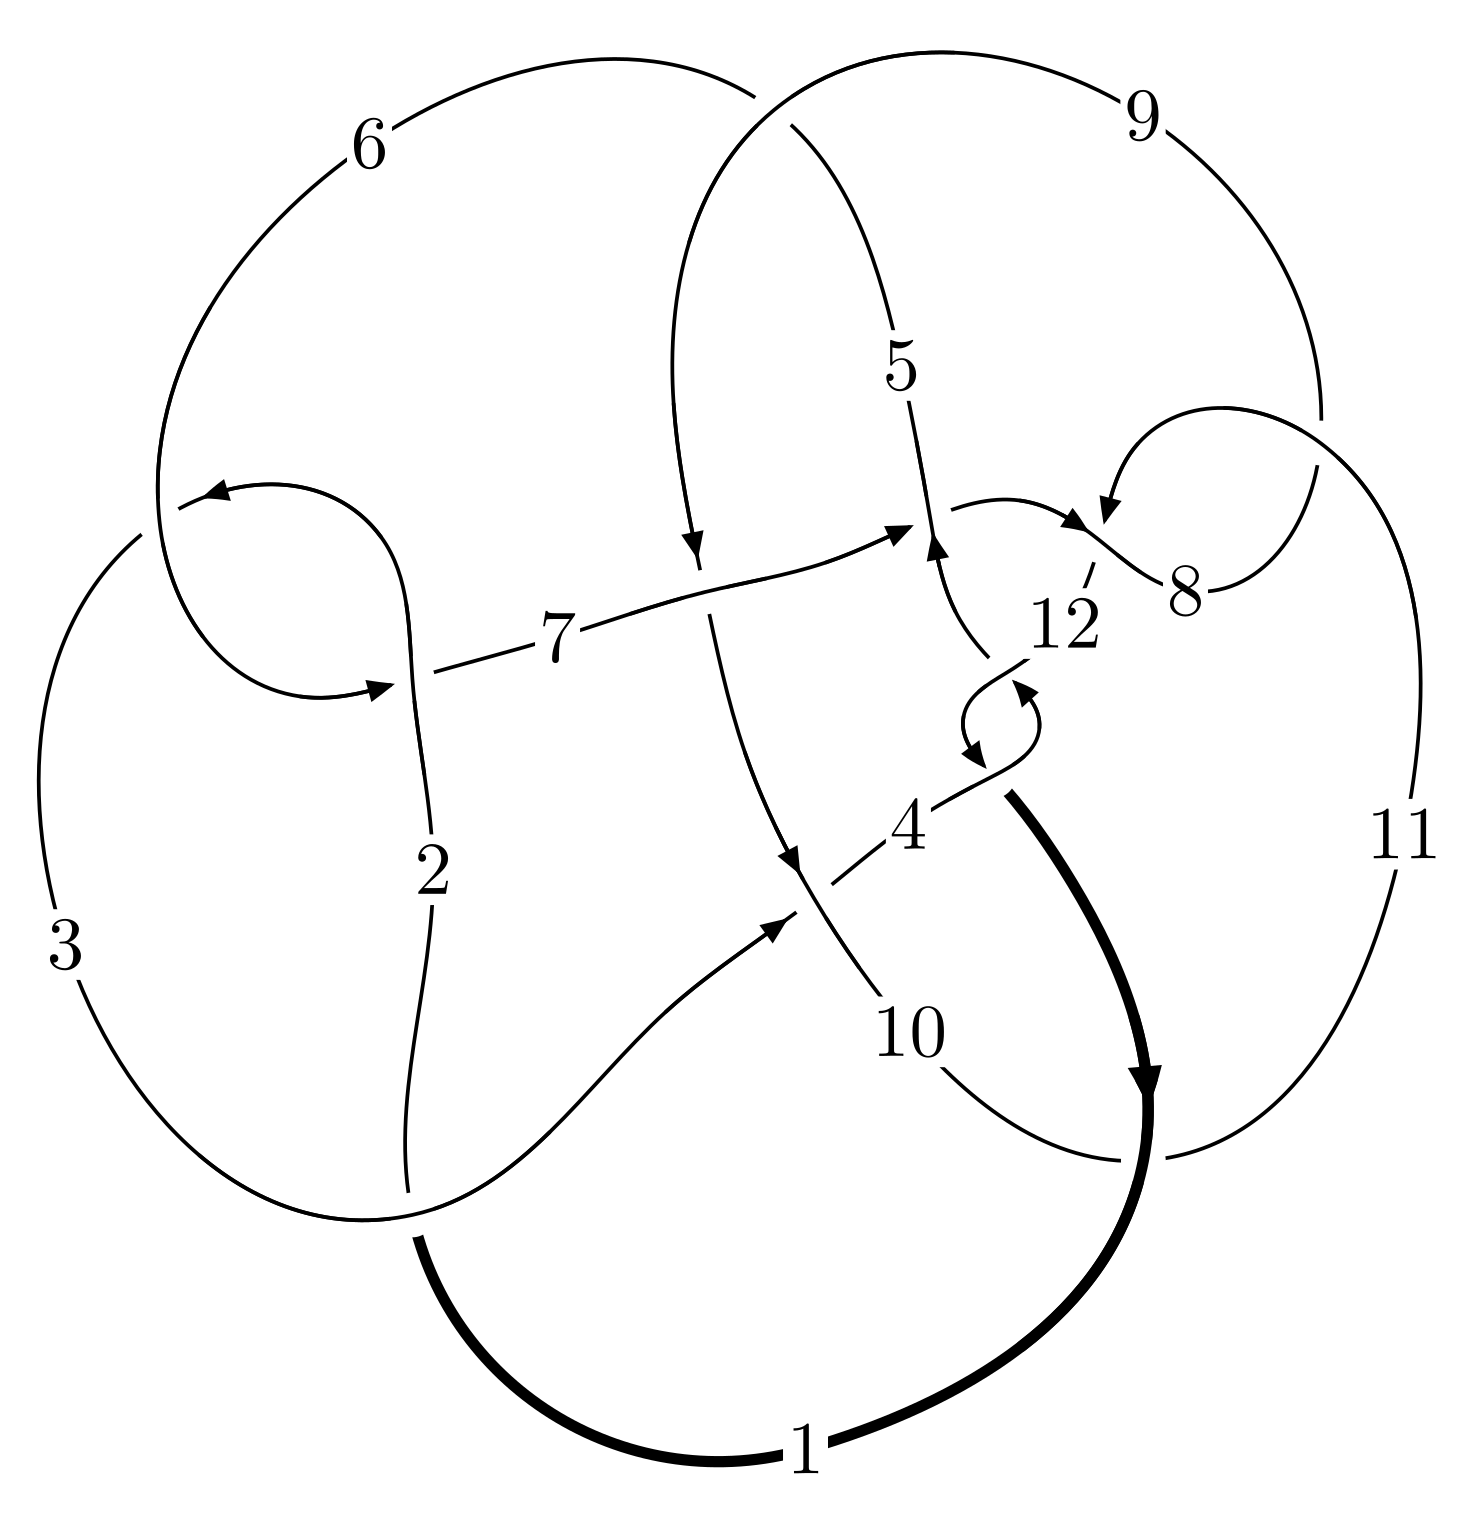
\includegraphics[width=112pt]{../../../GIT/diagram.site/Diagrams/png/1260_12a_0459.png}\\
\ \ \ A knot diagram\footnotemark}&
\allowdisplaybreaks
\textbf{Linearized knot diagam} \\
\cline{2-2}
 &
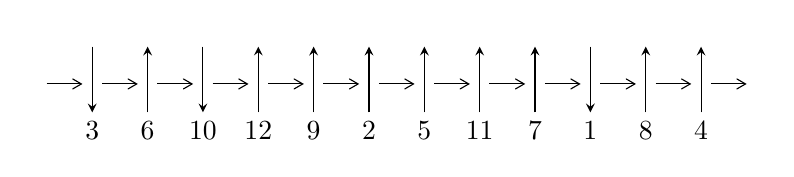
\begin{tikzpicture}[x=20pt, y=17pt]
	% nodes
	\node (C0) at (0, 0) {};
	\node (C1) at (1, 0) {};
	\node (C1U) at (1, +1) {};
	\node (C1D) at (1, -1) {3};

	\node (C2) at (2, 0) {};
	\node (C2U) at (2, +1) {};
	\node (C2D) at (2, -1) {6};

	\node (C3) at (3, 0) {};
	\node (C3U) at (3, +1) {};
	\node (C3D) at (3, -1) {10};

	\node (C4) at (4, 0) {};
	\node (C4U) at (4, +1) {};
	\node (C4D) at (4, -1) {12};

	\node (C5) at (5, 0) {};
	\node (C5U) at (5, +1) {};
	\node (C5D) at (5, -1) {9};

	\node (C6) at (6, 0) {};
	\node (C6U) at (6, +1) {};
	\node (C6D) at (6, -1) {2};

	\node (C7) at (7, 0) {};
	\node (C7U) at (7, +1) {};
	\node (C7D) at (7, -1) {5};

	\node (C8) at (8, 0) {};
	\node (C8U) at (8, +1) {};
	\node (C8D) at (8, -1) {11};

	\node (C9) at (9, 0) {};
	\node (C9U) at (9, +1) {};
	\node (C9D) at (9, -1) {7};

	\node (C10) at (10, 0) {};
	\node (C10U) at (10, +1) {};
	\node (C10D) at (10, -1) {1};

	\node (C11) at (11, 0) {};
	\node (C11U) at (11, +1) {};
	\node (C11D) at (11, -1) {8};

	\node (C12) at (12, 0) {};
	\node (C12U) at (12, +1) {};
	\node (C12D) at (12, -1) {4};
	\node (C13) at (13, 0) {};

	% arrows
	\draw[->,>={angle 60}]
	(C0) edge (C1) (C1) edge (C2) (C2) edge (C3) (C3) edge (C4) (C4) edge (C5) (C5) edge (C6) (C6) edge (C7) (C7) edge (C8) (C8) edge (C9) (C9) edge (C10) (C10) edge (C11) (C11) edge (C12) (C12) edge (C13) ;	\draw[->,>=stealth]
	(C1U) edge (C1D) (C2D) edge (C2U) (C3U) edge (C3D) (C4D) edge (C4U) (C5D) edge (C5U) (C6D) edge (C6U) (C7D) edge (C7U) (C8D) edge (C8U) (C9D) edge (C9U) (C10U) edge (C10D) (C11D) edge (C11U) (C12D) edge (C12U) ;
	\end{tikzpicture} \\
\hhline{~~} \\& 
\textbf{Solving Sequence} \\ \cline{2-2} 
 &
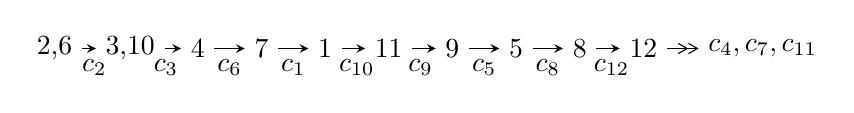
\begin{tikzpicture}[x=23pt, y=7pt]
	% node
	\node (A0) at (-1/8, 0) {2,6};
	\node (A1) at (17/16, 0) {3,10};
	\node (A2) at (17/8, 0) {4};
	\node (A3) at (25/8, 0) {7};
	\node (A4) at (33/8, 0) {1};
	\node (A5) at (41/8, 0) {11};
	\node (A6) at (49/8, 0) {9};
	\node (A7) at (57/8, 0) {5};
	\node (A8) at (65/8, 0) {8};
	\node (A9) at (73/8, 0) {12};
	\node (C1) at (1/2, -1) {$c_{2}$};
	\node (C2) at (13/8, -1) {$c_{3}$};
	\node (C3) at (21/8, -1) {$c_{6}$};
	\node (C4) at (29/8, -1) {$c_{1}$};
	\node (C5) at (37/8, -1) {$c_{10}$};
	\node (C6) at (45/8, -1) {$c_{9}$};
	\node (C7) at (53/8, -1) {$c_{5}$};
	\node (C8) at (61/8, -1) {$c_{8}$};
	\node (C9) at (69/8, -1) {$c_{12}$};
	\node (A10) at (11, 0) {$c_{4},c_{7},c_{11}$};

	% edge
	\draw[->,>=stealth]	
	(A0) edge (A1) (A1) edge (A2) (A2) edge (A3) (A3) edge (A4) (A4) edge (A5) (A5) edge (A6) (A6) edge (A7) (A7) edge (A8) (A8) edge (A9) ;
	\draw[->>,>={angle 60}]	
	(A9) edge (A10);
\end{tikzpicture} \\ 

\end{tabular} \\

\footnotetext{
The image of knot diagram is generated by the software ``\textbf{Draw programme}" developed by Andrew Bartholomew(\url{http://www.layer8.co.uk/maths/draw/index.htm\#Running-draw}), where we modified some parts for our purpose(\url{https://github.com/CATsTAILs/LinksPainter}).
}\phantom \\ \newline 
\centering \textbf{Ideals for irreducible components\footnotemark of $X_{\text{par}}$} 
 
\begin{align*}
I^u_{1}&=\langle 
7.16000\times10^{408} u^{158}+2.81310\times10^{409} u^{157}+\cdots+2.75929\times10^{409} b+1.24491\times10^{411},\\
\phantom{I^u_{1}}&\phantom{= \langle  }-4.54199\times10^{410} u^{158}-9.85253\times10^{410} u^{157}+\cdots+1.68317\times10^{411} a+9.52712\times10^{412},\\
\phantom{I^u_{1}}&\phantom{= \langle  }u^{159}+3 u^{158}+\cdots+254 u+61\rangle \\
I^u_{2}&=\langle 
1.89088\times10^{16} u^{37}+3.81587\times10^{16} u^{36}+\cdots+7.24163\times10^{15} b+3.77832\times10^{16},\\
\phantom{I^u_{2}}&\phantom{= \langle  }1.80953\times10^{15} u^{37}+7.77114\times10^{16} u^{36}+\cdots+2.17249\times10^{16} a+4.07624\times10^{17},\;u^{38}+2 u^{37}+\cdots+7 u+3\rangle \\
\\
\end{align*}
\raggedright * 2 irreducible components of $\dim_{\mathbb{C}}=0$, with total 197 representations.\\
\footnotetext{All coefficients of polynomials are rational numbers. But the coefficients are sometimes approximated in decimal forms when there is not enough margin.}
\newpage
\renewcommand{\arraystretch}{1}
\centering \section*{I. $I^u_{1}= \langle 7.16\times10^{408} u^{158}+2.81\times10^{409} u^{157}+\cdots+2.76\times10^{409} b+1.24\times10^{411},\;-4.54\times10^{410} u^{158}-9.85\times10^{410} u^{157}+\cdots+1.68\times10^{411} a+9.53\times10^{412},\;u^{159}+3 u^{158}+\cdots+254 u+61 \rangle$}
\flushleft \textbf{(i) Arc colorings}\\
\begin{tabular}{m{7pt} m{180pt} m{7pt} m{180pt} }
\flushright $a_{2}=$&$\begin{pmatrix}1\\0\end{pmatrix}$ \\
\flushright $a_{6}=$&$\begin{pmatrix}0\\u\end{pmatrix}$ \\
\flushright $a_{3}=$&$\begin{pmatrix}1\\- u^2\end{pmatrix}$ \\
\flushright $a_{10}=$&$\begin{pmatrix}0.269847 u^{158}+0.585356 u^{157}+\cdots-120.184 u-56.6022\\-0.259486 u^{158}-1.01950 u^{157}+\cdots-145.106 u-45.1168\end{pmatrix}$ \\
\flushright $a_{4}=$&$\begin{pmatrix}-1.65210 u^{158}-10.5481 u^{157}+\cdots-1632.96 u-475.800\\-1.25361 u^{158}-8.81070 u^{157}+\cdots-1243.70 u-384.679\end{pmatrix}$ \\
\flushright $a_{7}=$&$\begin{pmatrix}u\\u\end{pmatrix}$ \\
\flushright $a_{1}=$&$\begin{pmatrix}u^2+1\\- u^4\end{pmatrix}$ \\
\flushright $a_{11}=$&$\begin{pmatrix}-0.673257 u^{158}-2.06957 u^{157}+\cdots-302.818 u-99.0191\\-1.38391 u^{158}-3.80070 u^{157}+\cdots-335.208 u-87.9624\end{pmatrix}$ \\
\flushright $a_{9}=$&$\begin{pmatrix}-0.210299 u^{158}-0.627259 u^{157}+\cdots-156.754 u-57.6302\\-0.739633 u^{158}-2.23211 u^{157}+\cdots-181.676 u-46.1448\end{pmatrix}$ \\
\flushright $a_{5}=$&$\begin{pmatrix}-0.251684 u^{158}-5.77397 u^{157}+\cdots-1017.29 u-340.328\\-1.18463 u^{158}-7.36524 u^{157}+\cdots-1060.12 u-335.916\end{pmatrix}$ \\
\flushright $a_{8}=$&$\begin{pmatrix}2.71551 u^{158}+6.99494 u^{157}+\cdots+531.066 u+141.743\\1.99218 u^{158}+5.00541 u^{157}+\cdots+382.406 u+87.0731\end{pmatrix}$ \\
\flushright $a_{12}=$&$\begin{pmatrix}3.02859 u^{158}+7.14838 u^{157}+\cdots+521.124 u+129.485\\4.07615 u^{158}+10.0795 u^{157}+\cdots+726.211 u+149.463\end{pmatrix}$\\&\end{tabular}
\flushleft \textbf{(ii) Obstruction class $= -1$}\\~\\
\flushleft \textbf{(iii) Cusp Shapes $= 2.54355 u^{158}+4.06187 u^{157}+\cdots-159.678 u-151.190$}\\~\\
\newpage\renewcommand{\arraystretch}{1}
\flushleft \textbf{(iv) u-Polynomials at the component}\newline \\
\begin{tabular}{m{50pt}|m{274pt}}
Crossings & \hspace{64pt}u-Polynomials at each crossing \\
\hline $$\begin{aligned}c_{1}\end{aligned}$$&$\begin{aligned}
&u^{159}+63 u^{158}+\cdots-160940 u-3721
\end{aligned}$\\
\hline $$\begin{aligned}c_{2},c_{6}\end{aligned}$$&$\begin{aligned}
&u^{159}-3 u^{158}+\cdots+254 u-61
\end{aligned}$\\
\hline $$\begin{aligned}c_{3}\end{aligned}$$&$\begin{aligned}
&u^{159}+2 u^{158}+\cdots-6385 u-131
\end{aligned}$\\
\hline $$\begin{aligned}c_{4},c_{12}\end{aligned}$$&$\begin{aligned}
&u^{159}+6 u^{158}+\cdots+329355 u-46602
\end{aligned}$\\
\hline $$\begin{aligned}c_{5}\end{aligned}$$&$\begin{aligned}
&u^{159}-3 u^{158}+\cdots-31151 u-5272
\end{aligned}$\\
\hline $$\begin{aligned}c_{7}\end{aligned}$$&$\begin{aligned}
&u^{159}+13 u^{158}+\cdots-2559717451 u-258897949
\end{aligned}$\\
\hline $$\begin{aligned}c_{8},c_{11}\end{aligned}$$&$\begin{aligned}
&u^{159}-12 u^{158}+\cdots+5916498 u-656059
\end{aligned}$\\
\hline $$\begin{aligned}c_{9}\end{aligned}$$&$\begin{aligned}
&u^{159}+17 u^{158}+\cdots-44446 u-5041
\end{aligned}$\\
\hline $$\begin{aligned}c_{10}\end{aligned}$$&$\begin{aligned}
&u^{159}-16 u^{158}+\cdots+1503 u-71
\end{aligned}$\\
\hline
\end{tabular}\\~\\
\newpage\renewcommand{\arraystretch}{1}
\flushleft \textbf{(v) Riley Polynomials at the component}\newline \\
\begin{tabular}{m{50pt}|m{274pt}}
Crossings & \hspace{64pt}Riley Polynomials at each crossing \\
\hline $$\begin{aligned}c_{1}\end{aligned}$$&$\begin{aligned}
&y^{159}+63 y^{158}+\cdots+1061374132 y-13845841
\end{aligned}$\\
\hline $$\begin{aligned}c_{2},c_{6}\end{aligned}$$&$\begin{aligned}
&y^{159}+63 y^{158}+\cdots-160940 y-3721
\end{aligned}$\\
\hline $$\begin{aligned}c_{3}\end{aligned}$$&$\begin{aligned}
&y^{159}-8 y^{158}+\cdots+9604635 y-17161
\end{aligned}$\\
\hline $$\begin{aligned}c_{4},c_{12}\end{aligned}$$&$\begin{aligned}
&y^{159}+126 y^{158}+\cdots+236167644573 y-2171746404
\end{aligned}$\\
\hline $$\begin{aligned}c_{5}\end{aligned}$$&$\begin{aligned}
&y^{159}-15 y^{158}+\cdots-346128495 y-27793984
\end{aligned}$\\
\hline $$\begin{aligned}c_{7}\end{aligned}$$&$\begin{aligned}
&y^{159}+59 y^{158}+\cdots-1286314653118589129 y-67028147996406601
\end{aligned}$\\
\hline $$\begin{aligned}c_{8},c_{11}\end{aligned}$$&$\begin{aligned}
&y^{159}+102 y^{158}+\cdots-6052537066114 y-430413411481
\end{aligned}$\\
\hline $$\begin{aligned}c_{9}\end{aligned}$$&$\begin{aligned}
&y^{159}-9 y^{158}+\cdots+268040052 y-25411681
\end{aligned}$\\
\hline $$\begin{aligned}c_{10}\end{aligned}$$&$\begin{aligned}
&y^{159}-18 y^{158}+\cdots-151015 y-5041
\end{aligned}$\\
\hline
\end{tabular}\\~\\
\newpage\flushleft \textbf{(vi) Complex Volumes and Cusp Shapes}
$$\begin{array}{c|c|c}  
\text{Solutions to }I^u_{1}& \I (\text{vol} + \sqrt{-1}CS) & \text{Cusp shape}\\
 \hline 
\begin{aligned}
u &= \phantom{-}0.891606 + 0.451374 I \\
a &= -0.399037 - 0.880877 I \\
b &= -1.387810 + 0.079849 I\end{aligned}
 & -0.10649 - 4.58909 I & \phantom{-0.000000 } 0 \\ \hline\begin{aligned}
u &= \phantom{-}0.891606 - 0.451374 I \\
a &= -0.399037 + 0.880877 I \\
b &= -1.387810 - 0.079849 I\end{aligned}
 & -0.10649 + 4.58909 I & \phantom{-0.000000 } 0 \\ \hline\begin{aligned}
u &= \phantom{-}0.399869 + 0.927877 I \\
a &= \phantom{-}0.42775 - 2.20856 I \\
b &= -0.74809 - 2.12471 I\end{aligned}
 & -7.49146 + 2.95901 I & \phantom{-0.000000 } 0 \\ \hline\begin{aligned}
u &= \phantom{-}0.399869 - 0.927877 I \\
a &= \phantom{-}0.42775 + 2.20856 I \\
b &= -0.74809 + 2.12471 I\end{aligned}
 & -7.49146 - 2.95901 I & \phantom{-0.000000 } 0 \\ \hline\begin{aligned}
u &= -0.571758 + 0.834215 I \\
a &= \phantom{-}1.41778 - 0.73759 I \\
b &= \phantom{-}2.28792 - 0.39889 I\end{aligned}
 & \phantom{-}1.88865 - 1.06916 I & \phantom{-0.000000 } 0 \\ \hline\begin{aligned}
u &= -0.571758 - 0.834215 I \\
a &= \phantom{-}1.41778 + 0.73759 I \\
b &= \phantom{-}2.28792 + 0.39889 I\end{aligned}
 & \phantom{-}1.88865 + 1.06916 I & \phantom{-0.000000 } 0 \\ \hline\begin{aligned}
u &= \phantom{-}0.683602 + 0.708957 I \\
a &= \phantom{-}1.32111 - 0.58053 I \\
b &= \phantom{-}1.167530 - 0.538071 I\end{aligned}
 & -0.236758 - 1.021390 I & \phantom{-0.000000 } 0 \\ \hline\begin{aligned}
u &= \phantom{-}0.683602 - 0.708957 I \\
a &= \phantom{-}1.32111 + 0.58053 I \\
b &= \phantom{-}1.167530 + 0.538071 I\end{aligned}
 & -0.236758 + 1.021390 I & \phantom{-0.000000 } 0 \\ \hline\begin{aligned}
u &= \phantom{-}0.613617 + 0.809529 I \\
a &= -1.24201 - 1.46224 I \\
b &= -1.43474 + 0.13516 I\end{aligned}
 & \phantom{-}3.28186 + 0.91601 I & \phantom{-0.000000 } 0 \\ \hline\begin{aligned}
u &= \phantom{-}0.613617 - 0.809529 I \\
a &= -1.24201 + 1.46224 I \\
b &= -1.43474 - 0.13516 I\end{aligned}
 & \phantom{-}3.28186 - 0.91601 I & \phantom{-0.000000 } 0\\
 \hline 
 \end{array}$$\newpage$$\begin{array}{c|c|c}  
\text{Solutions to }I^u_{1}& \I (\text{vol} + \sqrt{-1}CS) & \text{Cusp shape}\\
 \hline 
\begin{aligned}
u &= \phantom{-}0.831614 + 0.498398 I \\
a &= \phantom{-}0.582103 + 0.698196 I \\
b &= \phantom{-}1.213780 + 0.049993 I\end{aligned}
 & \phantom{-}0.93629 - 3.11773 I & \phantom{-0.000000 } 0 \\ \hline\begin{aligned}
u &= \phantom{-}0.831614 - 0.498398 I \\
a &= \phantom{-}0.582103 - 0.698196 I \\
b &= \phantom{-}1.213780 - 0.049993 I\end{aligned}
 & \phantom{-}0.93629 + 3.11773 I & \phantom{-0.000000 } 0 \\ \hline\begin{aligned}
u &= -0.603720 + 0.758440 I \\
a &= -0.18923 + 1.77717 I \\
b &= -2.36106 + 1.11082 I\end{aligned}
 & -4.09868 + 4.78610 I & \phantom{-0.000000 } 0 \\ \hline\begin{aligned}
u &= -0.603720 - 0.758440 I \\
a &= -0.18923 - 1.77717 I \\
b &= -2.36106 - 1.11082 I\end{aligned}
 & -4.09868 - 4.78610 I & \phantom{-0.000000 } 0 \\ \hline\begin{aligned}
u &= -0.815510 + 0.510356 I \\
a &= -0.055289 - 1.063800 I \\
b &= \phantom{-}0.429918 - 0.267518 I\end{aligned}
 & \phantom{-}0.470123 - 0.643923 I & \phantom{-0.000000 } 0 \\ \hline\begin{aligned}
u &= -0.815510 - 0.510356 I \\
a &= -0.055289 + 1.063800 I \\
b &= \phantom{-}0.429918 + 0.267518 I\end{aligned}
 & \phantom{-}0.470123 + 0.643923 I & \phantom{-0.000000 } 0 \\ \hline\begin{aligned}
u &= -0.868748 + 0.576297 I \\
a &= \phantom{-}1.27606 - 0.87395 I \\
b &= \phantom{-}1.54440 + 0.59450 I\end{aligned}
 & -0.53884 + 7.54590 I & \phantom{-0.000000 } 0 \\ \hline\begin{aligned}
u &= -0.868748 - 0.576297 I \\
a &= \phantom{-}1.27606 + 0.87395 I \\
b &= \phantom{-}1.54440 - 0.59450 I\end{aligned}
 & -0.53884 - 7.54590 I & \phantom{-0.000000 } 0 \\ \hline\begin{aligned}
u &= -0.575233 + 0.869697 I \\
a &= \phantom{-}0.94013 - 2.21673 I \\
b &= \phantom{-}1.24916 - 1.17661 I\end{aligned}
 & \phantom{-}1.77261 - 3.50082 I & \phantom{-0.000000 } 0 \\ \hline\begin{aligned}
u &= -0.575233 - 0.869697 I \\
a &= \phantom{-}0.94013 + 2.21673 I \\
b &= \phantom{-}1.24916 + 1.17661 I\end{aligned}
 & \phantom{-}1.77261 + 3.50082 I & \phantom{-0.000000 } 0\\
 \hline 
 \end{array}$$\newpage$$\begin{array}{c|c|c}  
\text{Solutions to }I^u_{1}& \I (\text{vol} + \sqrt{-1}CS) & \text{Cusp shape}\\
 \hline 
\begin{aligned}
u &= \phantom{-}0.627251 + 0.721492 I \\
a &= \phantom{-}1.08372 + 2.32675 I \\
b &= \phantom{-}1.27777 + 1.06708 I\end{aligned}
 & -3.45995 - 5.36968 I & \phantom{-0.000000 } 0 \\ \hline\begin{aligned}
u &= \phantom{-}0.627251 - 0.721492 I \\
a &= \phantom{-}1.08372 - 2.32675 I \\
b &= \phantom{-}1.27777 - 1.06708 I\end{aligned}
 & -3.45995 + 5.36968 I & \phantom{-0.000000 } 0 \\ \hline\begin{aligned}
u &= \phantom{-}0.872842 + 0.574512 I \\
a &= -0.880043 - 0.920042 I \\
b &= -1.231380 + 0.332606 I\end{aligned}
 & \phantom{-}3.92115 - 3.61044 I & \phantom{-0.000000 } 0 \\ \hline\begin{aligned}
u &= \phantom{-}0.872842 - 0.574512 I \\
a &= -0.880043 + 0.920042 I \\
b &= -1.231380 - 0.332606 I\end{aligned}
 & \phantom{-}3.92115 + 3.61044 I & \phantom{-0.000000 } 0 \\ \hline\begin{aligned}
u &= -0.609586 + 0.849892 I \\
a &= \phantom{-}1.44685 - 2.54477 I \\
b &= \phantom{-}3.05712 - 0.70431 I\end{aligned}
 & \phantom{-}0.77339 - 2.40140 I & \phantom{-0.000000 } 0 \\ \hline\begin{aligned}
u &= -0.609586 - 0.849892 I \\
a &= \phantom{-}1.44685 + 2.54477 I \\
b &= \phantom{-}3.05712 + 0.70431 I\end{aligned}
 & \phantom{-}0.77339 + 2.40140 I & \phantom{-0.000000 } 0 \\ \hline\begin{aligned}
u &= -0.588733 + 0.750638 I \\
a &= -0.904183 + 0.740341 I \\
b &= -1.241650 + 0.556024 I\end{aligned}
 & \phantom{-}1.21651 - 1.58917 I & \phantom{-0.000000 } 0 \\ \hline\begin{aligned}
u &= -0.588733 - 0.750638 I \\
a &= -0.904183 - 0.740341 I \\
b &= -1.241650 - 0.556024 I\end{aligned}
 & \phantom{-}1.21651 + 1.58917 I & \phantom{-0.000000 } 0 \\ \hline\begin{aligned}
u &= -0.553031 + 0.767881 I \\
a &= -0.57305 + 1.84886 I \\
b &= -0.208333 + 0.772614 I\end{aligned}
 & -0.551910 + 1.122070 I & \phantom{-0.000000 } 0 \\ \hline\begin{aligned}
u &= -0.553031 - 0.767881 I \\
a &= -0.57305 - 1.84886 I \\
b &= -0.208333 - 0.772614 I\end{aligned}
 & -0.551910 - 1.122070 I & \phantom{-0.000000 } 0\\
 \hline 
 \end{array}$$\newpage$$\begin{array}{c|c|c}  
\text{Solutions to }I^u_{1}& \I (\text{vol} + \sqrt{-1}CS) & \text{Cusp shape}\\
 \hline 
\begin{aligned}
u &= \phantom{-}0.497138 + 0.802103 I \\
a &= \phantom{-}0.940684 + 0.349089 I \\
b &= -0.642794 - 0.744683 I\end{aligned}
 & -6.40496 + 2.25710 I & \phantom{-0.000000 } 0 \\ \hline\begin{aligned}
u &= \phantom{-}0.497138 - 0.802103 I \\
a &= \phantom{-}0.940684 - 0.349089 I \\
b &= -0.642794 + 0.744683 I\end{aligned}
 & -6.40496 - 2.25710 I & \phantom{-0.000000 } 0 \\ \hline\begin{aligned}
u &= \phantom{-}0.522717 + 0.918136 I \\
a &= -0.861764 - 0.279437 I \\
b &= \phantom{-}0.501977 + 0.832439 I\end{aligned}
 & -6.81443 + 1.89238 I & \phantom{-0.000000 } 0 \\ \hline\begin{aligned}
u &= \phantom{-}0.522717 - 0.918136 I \\
a &= -0.861764 + 0.279437 I \\
b &= \phantom{-}0.501977 - 0.832439 I\end{aligned}
 & -6.81443 - 1.89238 I & \phantom{-0.000000 } 0 \\ \hline\begin{aligned}
u &= \phantom{-}0.632740 + 0.847116 I \\
a &= -1.83466 - 2.13359 I \\
b &= -2.60512 - 1.20654 I\end{aligned}
 & \phantom{-}1.39791 + 2.47477 I & \phantom{-0.000000 } 0 \\ \hline\begin{aligned}
u &= \phantom{-}0.632740 - 0.847116 I \\
a &= -1.83466 + 2.13359 I \\
b &= -2.60512 + 1.20654 I\end{aligned}
 & \phantom{-}1.39791 - 2.47477 I & \phantom{-0.000000 } 0 \\ \hline\begin{aligned}
u &= \phantom{-}0.607609 + 0.711221 I \\
a &= -0.035942 + 0.740569 I \\
b &= \phantom{-}1.23958 + 0.90009 I\end{aligned}
 & \phantom{-}1.44425 - 1.69401 I & \phantom{-0.000000 } 0 \\ \hline\begin{aligned}
u &= \phantom{-}0.607609 - 0.711221 I \\
a &= -0.035942 - 0.740569 I \\
b &= \phantom{-}1.23958 - 0.90009 I\end{aligned}
 & \phantom{-}1.44425 + 1.69401 I & \phantom{-0.000000 } 0 \\ \hline\begin{aligned}
u &= \phantom{-}0.615466 + 0.873663 I \\
a &= -0.30344 - 1.40309 I \\
b &= -1.81053 - 1.19041 I\end{aligned}
 & \phantom{-}3.08306 + 3.92462 I & \phantom{-0.000000 } 0 \\ \hline\begin{aligned}
u &= \phantom{-}0.615466 - 0.873663 I \\
a &= -0.30344 + 1.40309 I \\
b &= -1.81053 + 1.19041 I\end{aligned}
 & \phantom{-}3.08306 - 3.92462 I & \phantom{-0.000000 } 0\\
 \hline 
 \end{array}$$\newpage$$\begin{array}{c|c|c}  
\text{Solutions to }I^u_{1}& \I (\text{vol} + \sqrt{-1}CS) & \text{Cusp shape}\\
 \hline 
\begin{aligned}
u &= -0.934127 + 0.528231 I \\
a &= -1.051730 + 0.882977 I \\
b &= -1.41419 - 0.55637 I\end{aligned}
 & -4.5491 + 14.0442 I & \phantom{-0.000000 } 0 \\ \hline\begin{aligned}
u &= -0.934127 - 0.528231 I \\
a &= -1.051730 - 0.882977 I \\
b &= -1.41419 + 0.55637 I\end{aligned}
 & -4.5491 - 14.0442 I & \phantom{-0.000000 } 0 \\ \hline\begin{aligned}
u &= -0.884763 + 0.265927 I \\
a &= -0.065974 + 0.990621 I \\
b &= -0.277394 + 0.133064 I\end{aligned}
 & \phantom{-}0.067585 - 0.143772 I & \phantom{-0.000000 } 0 \\ \hline\begin{aligned}
u &= -0.884763 - 0.265927 I \\
a &= -0.065974 - 0.990621 I \\
b &= -0.277394 - 0.133064 I\end{aligned}
 & \phantom{-}0.067585 + 0.143772 I & \phantom{-0.000000 } 0 \\ \hline\begin{aligned}
u &= \phantom{-}0.949654 + 0.508942 I \\
a &= \phantom{-}0.786316 + 0.857484 I \\
b &= \phantom{-}1.068240 - 0.317335 I\end{aligned}
 & \phantom{-}1.42546 - 7.94644 I & \phantom{-0.000000 } 0 \\ \hline\begin{aligned}
u &= \phantom{-}0.949654 - 0.508942 I \\
a &= \phantom{-}0.786316 - 0.857484 I \\
b &= \phantom{-}1.068240 + 0.317335 I\end{aligned}
 & \phantom{-}1.42546 + 7.94644 I & \phantom{-0.000000 } 0 \\ \hline\begin{aligned}
u &= -0.566757 + 0.921324 I \\
a &= -1.008770 - 0.000430 I \\
b &= -1.94280 + 0.18822 I\end{aligned}
 & -1.05014 - 5.62239 I & \phantom{-0.000000 } 0 \\ \hline\begin{aligned}
u &= -0.566757 - 0.921324 I \\
a &= -1.008770 + 0.000430 I \\
b &= -1.94280 - 0.18822 I\end{aligned}
 & -1.05014 + 5.62239 I & \phantom{-0.000000 } 0 \\ \hline\begin{aligned}
u &= -0.071453 + 1.082090 I \\
a &= -0.528626 + 0.466190 I \\
b &= \phantom{-}0.701369 - 0.226657 I\end{aligned}
 & -11.43230 + 0.10008 I & \phantom{-0.000000 } 0 \\ \hline\begin{aligned}
u &= -0.071453 - 1.082090 I \\
a &= -0.528626 - 0.466190 I \\
b &= \phantom{-}0.701369 + 0.226657 I\end{aligned}
 & -11.43230 - 0.10008 I & \phantom{-0.000000 } 0\\
 \hline 
 \end{array}$$\newpage$$\begin{array}{c|c|c}  
\text{Solutions to }I^u_{1}& \I (\text{vol} + \sqrt{-1}CS) & \text{Cusp shape}\\
 \hline 
\begin{aligned}
u &= -0.343598 + 0.842945 I \\
a &= \phantom{-}0.80711 - 1.83541 I \\
b &= \phantom{-}1.18296 - 1.98287 I\end{aligned}
 & -2.48699 + 1.18392 I & \phantom{-0.000000 } 0 \\ \hline\begin{aligned}
u &= -0.343598 - 0.842945 I \\
a &= \phantom{-}0.80711 + 1.83541 I \\
b &= \phantom{-}1.18296 + 1.98287 I\end{aligned}
 & -2.48699 - 1.18392 I & \phantom{-0.000000 } 0 \\ \hline\begin{aligned}
u &= -0.595995 + 0.919577 I \\
a &= -1.83619 + 1.92879 I \\
b &= -2.25512 - 0.32712 I\end{aligned}
 & -4.60052 - 9.53462 I & \phantom{-0.000000 } 0 \\ \hline\begin{aligned}
u &= -0.595995 - 0.919577 I \\
a &= -1.83619 - 1.92879 I \\
b &= -2.25512 + 0.32712 I\end{aligned}
 & -4.60052 + 9.53462 I & \phantom{-0.000000 } 0 \\ \hline\begin{aligned}
u &= -0.645641 + 0.628785 I \\
a &= \phantom{-}1.010270 - 0.702753 I \\
b &= \phantom{-}0.754803 + 1.111730 I\end{aligned}
 & -0.954940 + 0.088450 I & \phantom{-0.000000 } 0 \\ \hline\begin{aligned}
u &= -0.645641 - 0.628785 I \\
a &= \phantom{-}1.010270 + 0.702753 I \\
b &= \phantom{-}0.754803 - 1.111730 I\end{aligned}
 & -0.954940 - 0.088450 I & \phantom{-0.000000 } 0 \\ \hline\begin{aligned}
u &= -0.062257 + 1.101880 I \\
a &= \phantom{-}0.774289 + 0.733403 I \\
b &= -0.219207 + 0.885741 I\end{aligned}
 & -5.90968 - 1.00227 I & \phantom{-0.000000 } 0 \\ \hline\begin{aligned}
u &= -0.062257 - 1.101880 I \\
a &= \phantom{-}0.774289 - 0.733403 I \\
b &= -0.219207 - 0.885741 I\end{aligned}
 & -5.90968 + 1.00227 I & \phantom{-0.000000 } 0 \\ \hline\begin{aligned}
u &= -0.628272 + 0.908716 I \\
a &= -0.42968 + 1.46683 I \\
b &= -0.880148 + 1.051340 I\end{aligned}
 & \phantom{-}0.71583 - 3.24571 I & \phantom{-0.000000 } 0 \\ \hline\begin{aligned}
u &= -0.628272 - 0.908716 I \\
a &= -0.42968 - 1.46683 I \\
b &= -0.880148 - 1.051340 I\end{aligned}
 & \phantom{-}0.71583 + 3.24571 I & \phantom{-0.000000 } 0\\
 \hline 
 \end{array}$$\newpage$$\begin{array}{c|c|c}  
\text{Solutions to }I^u_{1}& \I (\text{vol} + \sqrt{-1}CS) & \text{Cusp shape}\\
 \hline 
\begin{aligned}
u &= \phantom{-}0.839307 + 0.294161 I \\
a &= \phantom{-}0.730632 - 0.193247 I \\
b &= \phantom{-}0.145461 - 0.690363 I\end{aligned}
 & -1.96454 + 3.63147 I & \phantom{-0.000000 } 0 \\ \hline\begin{aligned}
u &= \phantom{-}0.839307 - 0.294161 I \\
a &= \phantom{-}0.730632 + 0.193247 I \\
b &= \phantom{-}0.145461 + 0.690363 I\end{aligned}
 & -1.96454 - 3.63147 I & \phantom{-0.000000 } 0 \\ \hline\begin{aligned}
u &= \phantom{-}0.749765 + 0.825354 I \\
a &= -0.698807 + 1.067630 I \\
b &= \phantom{-}0.31282 + 1.42365 I\end{aligned}
 & -5.61660 + 0.32133 I & \phantom{-0.000000 } 0 \\ \hline\begin{aligned}
u &= \phantom{-}0.749765 - 0.825354 I \\
a &= -0.698807 - 1.067630 I \\
b &= \phantom{-}0.31282 - 1.42365 I\end{aligned}
 & -5.61660 - 0.32133 I & \phantom{-0.000000 } 0 \\ \hline\begin{aligned}
u &= -0.902924 + 0.660808 I \\
a &= -0.474272 + 0.497644 I \\
b &= -0.933594 - 0.010397 I\end{aligned}
 & \phantom{-}2.26957 - 2.33577 I & \phantom{-0.000000 } 0 \\ \hline\begin{aligned}
u &= -0.902924 - 0.660808 I \\
a &= -0.474272 - 0.497644 I \\
b &= -0.933594 + 0.010397 I\end{aligned}
 & \phantom{-}2.26957 + 2.33577 I & \phantom{-0.000000 } 0 \\ \hline\begin{aligned}
u &= \phantom{-}0.614092 + 0.936059 I \\
a &= \phantom{-}1.09199 + 1.04492 I \\
b &= \phantom{-}0.986717 - 0.242566 I\end{aligned}
 & \phantom{-}0.77023 + 6.53892 I & \phantom{-0.000000 } 0 \\ \hline\begin{aligned}
u &= \phantom{-}0.614092 - 0.936059 I \\
a &= \phantom{-}1.09199 - 1.04492 I \\
b &= \phantom{-}0.986717 + 0.242566 I\end{aligned}
 & \phantom{-}0.77023 - 6.53892 I & \phantom{-0.000000 } 0 \\ \hline\begin{aligned}
u &= \phantom{-}0.614061 + 0.939601 I \\
a &= \phantom{-}1.69890 + 1.00476 I \\
b &= \phantom{-}2.67904 + 0.70566 I\end{aligned}
 & -4.12502 + 10.25450 I & \phantom{-0.000000 } 0 \\ \hline\begin{aligned}
u &= \phantom{-}0.614061 - 0.939601 I \\
a &= \phantom{-}1.69890 - 1.00476 I \\
b &= \phantom{-}2.67904 - 0.70566 I\end{aligned}
 & -4.12502 - 10.25450 I & \phantom{-0.000000 } 0\\
 \hline 
 \end{array}$$\newpage$$\begin{array}{c|c|c}  
\text{Solutions to }I^u_{1}& \I (\text{vol} + \sqrt{-1}CS) & \text{Cusp shape}\\
 \hline 
\begin{aligned}
u &= \phantom{-}1.041450 + 0.419189 I \\
a &= -0.497265 + 0.333522 I \\
b &= \phantom{-}0.108138 + 0.587378 I\end{aligned}
 & -5.14019 + 8.67296 I & \phantom{-0.000000 } 0 \\ \hline\begin{aligned}
u &= \phantom{-}1.041450 - 0.419189 I \\
a &= -0.497265 - 0.333522 I \\
b &= \phantom{-}0.108138 - 0.587378 I\end{aligned}
 & -5.14019 - 8.67296 I & \phantom{-0.000000 } 0 \\ \hline\begin{aligned}
u &= -0.082693 + 1.123310 I \\
a &= -0.315749 + 0.112904 I \\
b &= \phantom{-}0.513951 + 0.319444 I\end{aligned}
 & -2.69089 - 2.42476 I & \phantom{-0.000000 } 0 \\ \hline\begin{aligned}
u &= -0.082693 - 1.123310 I \\
a &= -0.315749 - 0.112904 I \\
b &= \phantom{-}0.513951 - 0.319444 I\end{aligned}
 & -2.69089 + 2.42476 I & \phantom{-0.000000 } 0 \\ \hline\begin{aligned}
u &= -0.997319 + 0.525387 I \\
a &= \phantom{-}0.332017 - 0.391180 I \\
b &= \phantom{-}0.720221 + 0.183185 I\end{aligned}
 & \phantom{-}2.63643 + 1.45962 I & \phantom{-0.000000 } 0 \\ \hline\begin{aligned}
u &= -0.997319 - 0.525387 I \\
a &= \phantom{-}0.332017 + 0.391180 I \\
b &= \phantom{-}0.720221 - 0.183185 I\end{aligned}
 & \phantom{-}2.63643 - 1.45962 I & \phantom{-0.000000 } 0 \\ \hline\begin{aligned}
u &= \phantom{-}0.203757 + 1.109290 I \\
a &= \phantom{-}0.698695 + 0.024459 I \\
b &= -0.118743 - 0.669347 I\end{aligned}
 & -6.10046 - 0.54998 I & \phantom{-0.000000 } 0 \\ \hline\begin{aligned}
u &= \phantom{-}0.203757 - 1.109290 I \\
a &= \phantom{-}0.698695 - 0.024459 I \\
b &= -0.118743 + 0.669347 I\end{aligned}
 & -6.10046 + 0.54998 I & \phantom{-0.000000 } 0 \\ \hline\begin{aligned}
u &= -0.692665 + 0.521554 I \\
a &= -1.48146 + 1.30966 I \\
b &= -1.67966 - 0.21318 I\end{aligned}
 & -6.48598 + 1.52980 I & \phantom{-0.000000 } 0 \\ \hline\begin{aligned}
u &= -0.692665 - 0.521554 I \\
a &= -1.48146 - 1.30966 I \\
b &= -1.67966 + 0.21318 I\end{aligned}
 & -6.48598 - 1.52980 I & \phantom{-0.000000 } 0\\
 \hline 
 \end{array}$$\newpage$$\begin{array}{c|c|c}  
\text{Solutions to }I^u_{1}& \I (\text{vol} + \sqrt{-1}CS) & \text{Cusp shape}\\
 \hline 
\begin{aligned}
u &= \phantom{-}0.672646 + 0.935903 I \\
a &= -0.34462 + 1.54924 I \\
b &= -0.131100 + 1.395650 I\end{aligned}
 & -0.89825 + 6.26091 I & \phantom{-0.000000 } 0 \\ \hline\begin{aligned}
u &= \phantom{-}0.672646 - 0.935903 I \\
a &= -0.34462 - 1.54924 I \\
b &= -0.131100 - 1.395650 I\end{aligned}
 & -0.89825 - 6.26091 I & \phantom{-0.000000 } 0 \\ \hline\begin{aligned}
u &= -0.507923 + 1.036030 I \\
a &= -0.43365 + 2.07432 I \\
b &= -2.14224 + 1.26606 I\end{aligned}
 & -7.83347 - 9.11034 I & \phantom{-0.000000 } 0 \\ \hline\begin{aligned}
u &= -0.507923 - 1.036030 I \\
a &= -0.43365 - 2.07432 I \\
b &= -2.14224 - 1.26606 I\end{aligned}
 & -7.83347 + 9.11034 I & \phantom{-0.000000 } 0 \\ \hline\begin{aligned}
u &= \phantom{-}0.084320 + 1.162100 I \\
a &= \phantom{-}0.588540 - 0.162711 I \\
b &= -0.521174 + 0.170155 I\end{aligned}
 & -7.16691 + 6.22962 I & \phantom{-0.000000 } 0 \\ \hline\begin{aligned}
u &= \phantom{-}0.084320 - 1.162100 I \\
a &= \phantom{-}0.588540 + 0.162711 I \\
b &= -0.521174 - 0.170155 I\end{aligned}
 & -7.16691 - 6.22962 I & \phantom{-0.000000 } 0 \\ \hline\begin{aligned}
u &= -0.335652 + 0.764370 I \\
a &= -1.33194 + 2.73398 I \\
b &= -1.85917 + 0.24047 I\end{aligned}
 & -6.44396 + 5.52006 I & \phantom{-0.000000 } 0 \\ \hline\begin{aligned}
u &= -0.335652 - 0.764370 I \\
a &= -1.33194 - 2.73398 I \\
b &= -1.85917 - 0.24047 I\end{aligned}
 & -6.44396 - 5.52006 I & \phantom{-0.000000 } 0 \\ \hline\begin{aligned}
u &= \phantom{-}0.505247 + 1.053240 I \\
a &= -0.084250 + 1.129650 I \\
b &= \phantom{-}0.505172 + 1.124770 I\end{aligned}
 & -4.46368 + 1.07446 I & \phantom{-0.000000 } 0 \\ \hline\begin{aligned}
u &= \phantom{-}0.505247 - 1.053240 I \\
a &= -0.084250 - 1.129650 I \\
b &= \phantom{-}0.505172 - 1.124770 I\end{aligned}
 & -4.46368 - 1.07446 I & \phantom{-0.000000 } 0\\
 \hline 
 \end{array}$$\newpage$$\begin{array}{c|c|c}  
\text{Solutions to }I^u_{1}& \I (\text{vol} + \sqrt{-1}CS) & \text{Cusp shape}\\
 \hline 
\begin{aligned}
u &= \phantom{-}0.214743 + 1.149270 I \\
a &= \phantom{-}0.128211 - 0.777716 I \\
b &= \phantom{-}1.037460 - 0.532001 I\end{aligned}
 & -10.79030 - 3.03275 I & \phantom{-0.000000 } 0 \\ \hline\begin{aligned}
u &= \phantom{-}0.214743 - 1.149270 I \\
a &= \phantom{-}0.128211 + 0.777716 I \\
b &= \phantom{-}1.037460 + 0.532001 I\end{aligned}
 & -10.79030 + 3.03275 I & \phantom{-0.000000 } 0 \\ \hline\begin{aligned}
u &= -0.329478 + 1.125570 I \\
a &= -1.41147 - 0.19219 I \\
b &= -0.564611 - 1.189060 I\end{aligned}
 & -8.97038 + 2.08423 I & \phantom{-0.000000 } 0 \\ \hline\begin{aligned}
u &= -0.329478 - 1.125570 I \\
a &= -1.41147 + 0.19219 I \\
b &= -0.564611 + 1.189060 I\end{aligned}
 & -8.97038 - 2.08423 I & \phantom{-0.000000 } 0 \\ \hline\begin{aligned}
u &= \phantom{-}0.573234 + 1.034610 I \\
a &= \phantom{-}0.66515 + 1.81424 I \\
b &= \phantom{-}2.00514 + 1.32017 I\end{aligned}
 & -3.73577 + 7.30425 I & \phantom{-0.000000 } 0 \\ \hline\begin{aligned}
u &= \phantom{-}0.573234 - 1.034610 I \\
a &= \phantom{-}0.66515 - 1.81424 I \\
b &= \phantom{-}2.00514 - 1.32017 I\end{aligned}
 & -3.73577 - 7.30425 I & \phantom{-0.000000 } 0 \\ \hline\begin{aligned}
u &= -0.626228 + 1.010830 I \\
a &= \phantom{-}0.585336 - 0.050441 I \\
b &= \phantom{-}1.185370 + 0.011923 I\end{aligned}
 & -1.08115 - 4.55575 I & \phantom{-0.000000 } 0 \\ \hline\begin{aligned}
u &= -0.626228 - 1.010830 I \\
a &= \phantom{-}0.585336 + 0.050441 I \\
b &= \phantom{-}1.185370 - 0.011923 I\end{aligned}
 & -1.08115 + 4.55575 I & \phantom{-0.000000 } 0 \\ \hline\begin{aligned}
u &= \phantom{-}0.553152 + 1.052900 I \\
a &= -0.78032 - 1.85728 I \\
b &= -1.28934 - 1.88716 I\end{aligned}
 & -8.64744 + 10.19800 I & \phantom{-0.000000 } 0 \\ \hline\begin{aligned}
u &= \phantom{-}0.553152 - 1.052900 I \\
a &= -0.78032 + 1.85728 I \\
b &= -1.28934 + 1.88716 I\end{aligned}
 & -8.64744 - 10.19800 I & \phantom{-0.000000 } 0\\
 \hline 
 \end{array}$$\newpage$$\begin{array}{c|c|c}  
\text{Solutions to }I^u_{1}& \I (\text{vol} + \sqrt{-1}CS) & \text{Cusp shape}\\
 \hline 
\begin{aligned}
u &= -0.670451 + 0.984890 I \\
a &= -0.489466 - 1.085880 I \\
b &= \phantom{-}0.92873 - 1.45141 I\end{aligned}
 & -1.96691 - 5.24950 I & \phantom{-0.000000 } 0 \\ \hline\begin{aligned}
u &= -0.670451 - 0.984890 I \\
a &= -0.489466 + 1.085880 I \\
b &= \phantom{-}0.92873 + 1.45141 I\end{aligned}
 & -1.96691 + 5.24950 I & \phantom{-0.000000 } 0 \\ \hline\begin{aligned}
u &= -0.457777 + 1.104550 I \\
a &= \phantom{-}0.929703 - 0.845257 I \\
b &= \phantom{-}1.31324 - 0.91960 I\end{aligned}
 & -3.73394 - 3.95029 I & \phantom{-0.000000 } 0 \\ \hline\begin{aligned}
u &= -0.457777 - 1.104550 I \\
a &= \phantom{-}0.929703 + 0.845257 I \\
b &= \phantom{-}1.31324 + 0.91960 I\end{aligned}
 & -3.73394 + 3.95029 I & \phantom{-0.000000 } 0 \\ \hline\begin{aligned}
u &= -0.388814 + 0.700087 I \\
a &= -0.23567 - 1.72227 I \\
b &= -0.116076 - 0.547040 I\end{aligned}
 & \phantom{-}0.453064 + 0.029676 I & \phantom{-0.000000 } 0 \\ \hline\begin{aligned}
u &= -0.388814 - 0.700087 I \\
a &= -0.23567 + 1.72227 I \\
b &= -0.116076 + 0.547040 I\end{aligned}
 & \phantom{-}0.453064 - 0.029676 I & \phantom{-0.000000 } 0 \\ \hline\begin{aligned}
u &= -0.623240 + 1.038110 I \\
a &= -0.73855 + 2.19114 I \\
b &= -2.03884 + 1.84794 I\end{aligned}
 & -7.97107 - 6.62345 I & \phantom{-0.000000 } 0 \\ \hline\begin{aligned}
u &= -0.623240 - 1.038110 I \\
a &= -0.73855 - 2.19114 I \\
b &= -2.03884 - 1.84794 I\end{aligned}
 & -7.97107 + 6.62345 I & \phantom{-0.000000 } 0 \\ \hline\begin{aligned}
u &= \phantom{-}0.114628 + 1.238640 I \\
a &= -0.772355 - 0.165121 I \\
b &= -0.463441 + 0.435036 I\end{aligned}
 & -6.04736 - 1.91666 I & \phantom{-0.000000 } 0 \\ \hline\begin{aligned}
u &= \phantom{-}0.114628 - 1.238640 I \\
a &= -0.772355 + 0.165121 I \\
b &= -0.463441 - 0.435036 I\end{aligned}
 & -6.04736 + 1.91666 I & \phantom{-0.000000 } 0\\
 \hline 
 \end{array}$$\newpage$$\begin{array}{c|c|c}  
\text{Solutions to }I^u_{1}& \I (\text{vol} + \sqrt{-1}CS) & \text{Cusp shape}\\
 \hline 
\begin{aligned}
u &= -0.708136 + 1.032670 I \\
a &= -0.388373 + 1.181580 I \\
b &= -1.082470 + 0.876189 I\end{aligned}
 & \phantom{-}1.09638 - 3.58717 I & \phantom{-0.000000 } 0 \\ \hline\begin{aligned}
u &= -0.708136 - 1.032670 I \\
a &= -0.388373 - 1.181580 I \\
b &= -1.082470 - 0.876189 I\end{aligned}
 & \phantom{-}1.09638 + 3.58717 I & \phantom{-0.000000 } 0 \\ \hline\begin{aligned}
u &= \phantom{-}0.219256 + 0.706031 I \\
a &= -1.73960 - 0.66953 I \\
b &= -1.51753 - 1.35320 I\end{aligned}
 & -6.65955 - 6.15096 I & \phantom{-0.000000 } 0 \\ \hline\begin{aligned}
u &= \phantom{-}0.219256 - 0.706031 I \\
a &= -1.73960 + 0.66953 I \\
b &= -1.51753 + 1.35320 I\end{aligned}
 & -6.65955 + 6.15096 I & \phantom{-0.000000 } 0 \\ \hline\begin{aligned}
u &= \phantom{-}0.777772 + 0.994883 I \\
a &= \phantom{-}0.796367 - 0.675047 I \\
b &= \phantom{-}0.218636 - 1.334040 I\end{aligned}
 & -6.09025 + 5.57926 I & \phantom{-0.000000 } 0 \\ \hline\begin{aligned}
u &= \phantom{-}0.777772 - 0.994883 I \\
a &= \phantom{-}0.796367 + 0.675047 I \\
b &= \phantom{-}0.218636 + 1.334040 I\end{aligned}
 & -6.09025 - 5.57926 I & \phantom{-0.000000 } 0 \\ \hline\begin{aligned}
u &= -1.247940 + 0.246837 I \\
a &= \phantom{-}0.042339 - 0.161157 I \\
b &= \phantom{-}0.075085 + 0.245060 I\end{aligned}
 & \phantom{-}1.02894 - 1.15088 I & \phantom{-0.000000 } 0 \\ \hline\begin{aligned}
u &= -1.247940 - 0.246837 I \\
a &= \phantom{-}0.042339 + 0.161157 I \\
b &= \phantom{-}0.075085 - 0.245060 I\end{aligned}
 & \phantom{-}1.02894 + 1.15088 I & \phantom{-0.000000 } 0 \\ \hline\begin{aligned}
u &= \phantom{-}0.076094 + 1.271130 I \\
a &= \phantom{-}0.560911 + 0.294765 I \\
b &= \phantom{-}0.122577 + 0.139020 I\end{aligned}
 & -4.97447 - 0.78694 I & \phantom{-0.000000 } 0 \\ \hline\begin{aligned}
u &= \phantom{-}0.076094 - 1.271130 I \\
a &= \phantom{-}0.560911 - 0.294765 I \\
b &= \phantom{-}0.122577 - 0.139020 I\end{aligned}
 & -4.97447 + 0.78694 I & \phantom{-0.000000 } 0\\
 \hline 
 \end{array}$$\newpage$$\begin{array}{c|c|c}  
\text{Solutions to }I^u_{1}& \I (\text{vol} + \sqrt{-1}CS) & \text{Cusp shape}\\
 \hline 
\begin{aligned}
u &= \phantom{-}0.066043 + 1.273770 I \\
a &= -0.451108 + 0.114589 I \\
b &= \phantom{-}0.453927 - 0.297525 I\end{aligned}
 & -11.5403 + 11.8535 I & \phantom{-0.000000 } 0 \\ \hline\begin{aligned}
u &= \phantom{-}0.066043 - 1.273770 I \\
a &= -0.451108 - 0.114589 I \\
b &= \phantom{-}0.453927 + 0.297525 I\end{aligned}
 & -11.5403 - 11.8535 I & \phantom{-0.000000 } 0 \\ \hline\begin{aligned}
u &= \phantom{-}0.662213 + 1.093830 I \\
a &= \phantom{-}0.65581 + 1.44233 I \\
b &= \phantom{-}1.41474 + 0.96411 I\end{aligned}
 & -0.84101 + 8.70296 I & \phantom{-0.000000 } 0 \\ \hline\begin{aligned}
u &= \phantom{-}0.662213 - 1.093830 I \\
a &= \phantom{-}0.65581 - 1.44233 I \\
b &= \phantom{-}1.41474 - 0.96411 I\end{aligned}
 & -0.84101 - 8.70296 I & \phantom{-0.000000 } 0 \\ \hline\begin{aligned}
u &= \phantom{-}0.693099 + 1.078350 I \\
a &= -0.51511 - 1.54099 I \\
b &= -1.71907 - 1.32929 I\end{aligned}
 & \phantom{-}2.37709 + 9.41632 I & \phantom{-0.000000 } 0 \\ \hline\begin{aligned}
u &= \phantom{-}0.693099 - 1.078350 I \\
a &= -0.51511 + 1.54099 I \\
b &= -1.71907 + 1.32929 I\end{aligned}
 & \phantom{-}2.37709 - 9.41632 I & \phantom{-0.000000 } 0 \\ \hline\begin{aligned}
u &= -0.695608 + 1.077510 I \\
a &= \phantom{-}0.44958 - 1.96324 I \\
b &= \phantom{-}1.82591 - 1.76850 I\end{aligned}
 & -2.06941 - 13.35370 I & \phantom{-0.000000 } 0 \\ \hline\begin{aligned}
u &= -0.695608 - 1.077510 I \\
a &= \phantom{-}0.44958 + 1.96324 I \\
b &= \phantom{-}1.82591 + 1.76850 I\end{aligned}
 & -2.06941 + 13.35370 I & \phantom{-0.000000 } 0 \\ \hline\begin{aligned}
u &= \phantom{-}0.660840 + 1.135020 I \\
a &= -0.79320 - 1.45488 I \\
b &= -1.78706 - 0.78397 I\end{aligned}
 & -2.17517 + 10.31870 I & \phantom{-0.000000 } 0 \\ \hline\begin{aligned}
u &= \phantom{-}0.660840 - 1.135020 I \\
a &= -0.79320 + 1.45488 I \\
b &= -1.78706 + 0.78397 I\end{aligned}
 & -2.17517 - 10.31870 I & \phantom{-0.000000 } 0\\
 \hline 
 \end{array}$$\newpage$$\begin{array}{c|c|c}  
\text{Solutions to }I^u_{1}& \I (\text{vol} + \sqrt{-1}CS) & \text{Cusp shape}\\
 \hline 
\begin{aligned}
u &= -0.699736 + 1.120050 I \\
a &= -0.52746 + 1.79089 I \\
b &= -1.86336 + 1.59857 I\end{aligned}
 & -6.3731 - 20.0336 I & \phantom{-0.000000 } 0 \\ \hline\begin{aligned}
u &= -0.699736 - 1.120050 I \\
a &= -0.52746 - 1.79089 I \\
b &= -1.86336 - 1.59857 I\end{aligned}
 & -6.3731 + 20.0336 I & \phantom{-0.000000 } 0 \\ \hline\begin{aligned}
u &= -0.082018 + 1.320590 I \\
a &= \phantom{-}0.0961673 + 0.0711012 I \\
b &= -0.621161 - 0.145846 I\end{aligned}
 & -5.70638 - 5.46309 I & \phantom{-0.000000 } 0 \\ \hline\begin{aligned}
u &= -0.082018 - 1.320590 I \\
a &= \phantom{-}0.0961673 - 0.0711012 I \\
b &= -0.621161 + 0.145846 I\end{aligned}
 & -5.70638 + 5.46309 I & \phantom{-0.000000 } 0 \\ \hline\begin{aligned}
u &= \phantom{-}0.698089 + 1.129470 I \\
a &= \phantom{-}0.56404 + 1.41401 I \\
b &= \phantom{-}1.67719 + 1.30711 I\end{aligned}
 & -0.48522 + 13.96210 I & \phantom{-0.000000 } 0 \\ \hline\begin{aligned}
u &= \phantom{-}0.698089 - 1.129470 I \\
a &= \phantom{-}0.56404 - 1.41401 I \\
b &= \phantom{-}1.67719 - 1.30711 I\end{aligned}
 & -0.48522 - 13.96210 I & \phantom{-0.000000 } 0 \\ \hline\begin{aligned}
u &= -0.716426 + 1.132810 I \\
a &= \phantom{-}0.320924 - 1.047460 I \\
b &= \phantom{-}1.090520 - 0.822092 I\end{aligned}
 & \phantom{-}0.74553 - 7.64812 I & \phantom{-0.000000 } 0 \\ \hline\begin{aligned}
u &= -0.716426 - 1.132810 I \\
a &= \phantom{-}0.320924 + 1.047460 I \\
b &= \phantom{-}1.090520 + 0.822092 I\end{aligned}
 & \phantom{-}0.74553 + 7.64812 I & \phantom{-0.000000 } 0 \\ \hline\begin{aligned}
u &= -0.737999 + 1.123130 I \\
a &= \phantom{-}0.099504 - 0.680268 I \\
b &= \phantom{-}1.002420 - 0.822822 I\end{aligned}
 & -1.62771 - 5.11952 I & \phantom{-0.000000 } 0 \\ \hline\begin{aligned}
u &= -0.737999 - 1.123130 I \\
a &= \phantom{-}0.099504 + 0.680268 I \\
b &= \phantom{-}1.002420 + 0.822822 I\end{aligned}
 & -1.62771 + 5.11952 I & \phantom{-0.000000 } 0\\
 \hline 
 \end{array}$$\newpage$$\begin{array}{c|c|c}  
\text{Solutions to }I^u_{1}& \I (\text{vol} + \sqrt{-1}CS) & \text{Cusp shape}\\
 \hline 
\begin{aligned}
u &= \phantom{-}0.498926 + 0.404048 I \\
a &= \phantom{-}0.57619 + 1.82941 I \\
b &= \phantom{-}1.200400 - 0.049494 I\end{aligned}
 & -2.11405 - 2.75941 I & \phantom{-}3.06383 + 4.92986 I \\ \hline\begin{aligned}
u &= \phantom{-}0.498926 - 0.404048 I \\
a &= \phantom{-}0.57619 - 1.82941 I \\
b &= \phantom{-}1.200400 + 0.049494 I\end{aligned}
 & -2.11405 + 2.75941 I & \phantom{-}3.06383 - 4.92986 I \\ \hline\begin{aligned}
u &= \phantom{-}0.353254 + 0.524132 I \\
a &= -1.98450 + 0.75608 I \\
b &= -0.65495 + 1.30072 I\end{aligned}
 & -6.43990 + 0.21273 I & \phantom{-}2.10466 - 2.88222 I \\ \hline\begin{aligned}
u &= \phantom{-}0.353254 - 0.524132 I \\
a &= -1.98450 - 0.75608 I \\
b &= -0.65495 - 1.30072 I\end{aligned}
 & -6.43990 - 0.21273 I & \phantom{-}2.10466 + 2.88222 I \\ \hline\begin{aligned}
u &= \phantom{-}0.579950 + 0.243442 I \\
a &= -1.64163 - 1.20353 I \\
b &= -0.869948 - 0.299649 I\end{aligned}
 & -6.67361 - 5.76857 I & \phantom{-}1.19700 + 3.98730 I \\ \hline\begin{aligned}
u &= \phantom{-}0.579950 - 0.243442 I \\
a &= -1.64163 + 1.20353 I \\
b &= -0.869948 + 0.299649 I\end{aligned}
 & -6.67361 + 5.76857 I & \phantom{-}1.19700 - 3.98730 I \\ \hline\begin{aligned}
u &= \phantom{-}0.574453 + 1.262280 I \\
a &= \phantom{-}0.031831 - 0.594807 I \\
b &= -0.204980 - 0.761417 I\end{aligned}
 & -8.02830 - 2.54868 I & \phantom{-0.000000 } 0 \\ \hline\begin{aligned}
u &= \phantom{-}0.574453 - 1.262280 I \\
a &= \phantom{-}0.031831 + 0.594807 I \\
b &= -0.204980 + 0.761417 I\end{aligned}
 & -8.02830 + 2.54868 I & \phantom{-0.000000 } 0 \\ \hline\begin{aligned}
u &= -0.673803 + 1.220830 I \\
a &= -0.428510 + 0.652156 I \\
b &= -1.22811 + 0.78321 I\end{aligned}
 & -2.75965 - 5.66705 I & \phantom{-0.000000 } 0 \\ \hline\begin{aligned}
u &= -0.673803 - 1.220830 I \\
a &= -0.428510 - 0.652156 I \\
b &= -1.22811 - 0.78321 I\end{aligned}
 & -2.75965 + 5.66705 I & \phantom{-0.000000 } 0\\
 \hline 
 \end{array}$$\newpage$$\begin{array}{c|c|c}  
\text{Solutions to }I^u_{1}& \I (\text{vol} + \sqrt{-1}CS) & \text{Cusp shape}\\
 \hline 
\begin{aligned}
u &= \phantom{-}0.148298 + 0.538013 I \\
a &= \phantom{-}1.18272 + 2.36230 I \\
b &= \phantom{-}1.001110 + 0.458544 I\end{aligned}
 & -2.03542 - 2.73997 I & \phantom{-}1.46092 + 6.56987 I \\ \hline\begin{aligned}
u &= \phantom{-}0.148298 - 0.538013 I \\
a &= \phantom{-}1.18272 - 2.36230 I \\
b &= \phantom{-}1.001110 - 0.458544 I\end{aligned}
 & -2.03542 + 2.73997 I & \phantom{-}1.46092 - 6.56987 I \\ \hline\begin{aligned}
u &= -0.528592 + 0.033707 I \\
a &= \phantom{-}1.07746 + 1.02503 I \\
b &= -1.050220 - 0.728367 I\end{aligned}
 & -5.67142 + 5.34232 I & \phantom{-}1.94062 - 3.00311 I \\ \hline\begin{aligned}
u &= -0.528592 - 0.033707 I \\
a &= \phantom{-}1.07746 - 1.02503 I \\
b &= -1.050220 + 0.728367 I\end{aligned}
 & -5.67142 - 5.34232 I & \phantom{-}1.94062 + 3.00311 I \\ \hline\begin{aligned}
u &= -0.105801 + 0.462126 I \\
a &= \phantom{-}1.21181 - 1.85711 I \\
b &= \phantom{-}0.806452 + 0.797118 I\end{aligned}
 & -1.237960 - 0.251521 I & \phantom{-}2.04267 - 1.76475 I \\ \hline\begin{aligned}
u &= -0.105801 - 0.462126 I \\
a &= \phantom{-}1.21181 + 1.85711 I \\
b &= \phantom{-}0.806452 - 0.797118 I\end{aligned}
 & -1.237960 + 0.251521 I & \phantom{-}2.04267 + 1.76475 I \\ \hline\begin{aligned}
u &= -0.411659\phantom{ +0.000000I} \\
a &= -1.64181\phantom{ +0.000000I} \\
b &= -0.0904021\phantom{ +0.000000I}\end{aligned}
 & \phantom{-}1.01780\phantom{ +0.000000I} & \phantom{-}9.02240\phantom{ +0.000000I} \\ \hline\begin{aligned}
u &= -0.098178 + 0.385659 I \\
a &= -0.750766 + 0.834728 I \\
b &= \phantom{-}0.155455 + 0.915784 I\end{aligned}
 & \phantom{-}0.53987 - 1.41440 I & \phantom{-}3.09127 + 6.46715 I \\ \hline\begin{aligned}
u &= -0.098178 - 0.385659 I \\
a &= -0.750766 - 0.834728 I \\
b &= \phantom{-}0.155455 - 0.915784 I\end{aligned}
 & \phantom{-}0.53987 + 1.41440 I & \phantom{-}3.09127 - 6.46715 I\\
 \hline 
 \end{array}$$\newpage\newpage\renewcommand{\arraystretch}{1}
\centering \section*{II. $I^u_{2}= \langle 1.89\times10^{16} u^{37}+3.82\times10^{16} u^{36}+\cdots+7.24\times10^{15} b+3.78\times10^{16},\;1.81\times10^{15} u^{37}+7.77\times10^{16} u^{36}+\cdots+2.17\times10^{16} a+4.08\times10^{17},\;u^{38}+2 u^{37}+\cdots+7 u+3 \rangle$}
\flushleft \textbf{(i) Arc colorings}\\
\begin{tabular}{m{7pt} m{180pt} m{7pt} m{180pt} }
\flushright $a_{2}=$&$\begin{pmatrix}1\\0\end{pmatrix}$ \\
\flushright $a_{6}=$&$\begin{pmatrix}0\\u\end{pmatrix}$ \\
\flushright $a_{3}=$&$\begin{pmatrix}1\\- u^2\end{pmatrix}$ \\
\flushright $a_{10}=$&$\begin{pmatrix}-0.0832929 u^{37}-3.57707 u^{36}+\cdots-35.1519 u-18.7630\\-2.61112 u^{37}-5.26936 u^{36}+\cdots-13.8591 u-5.21751\end{pmatrix}$ \\
\flushright $a_{4}=$&$\begin{pmatrix}-1.46042 u^{37}-4.41875 u^{36}+\cdots-30.7239 u-10.2685\\-1.24772 u^{37}-2.76294 u^{36}+\cdots-20.5806 u-7.40635\end{pmatrix}$ \\
\flushright $a_{7}=$&$\begin{pmatrix}u\\u\end{pmatrix}$ \\
\flushright $a_{1}=$&$\begin{pmatrix}u^2+1\\- u^4\end{pmatrix}$ \\
\flushright $a_{11}=$&$\begin{pmatrix}-0.898685 u^{37}-4.45538 u^{36}+\cdots-28.6677 u-13.7937\\-5.67118 u^{37}-11.2912 u^{36}+\cdots-25.4961 u-6.24631\end{pmatrix}$ \\
\flushright $a_{9}=$&$\begin{pmatrix}-1.15463 u^{37}-3.68950 u^{36}+\cdots-19.1918 u-8.67288\\-3.68245 u^{37}-5.38179 u^{36}+\cdots+2.10103 u+4.87260\end{pmatrix}$ \\
\flushright $a_{5}=$&$\begin{pmatrix}-0.224924 u^{37}-2.18109 u^{36}+\cdots-19.6681 u-12.6508\\-0.852294 u^{37}-4.02176 u^{36}+\cdots-18.1714 u-10.7044\end{pmatrix}$ \\
\flushright $a_{8}=$&$\begin{pmatrix}-0.448661 u^{37}-2.86350 u^{36}+\cdots-10.0284 u-4.39321\\-2.39818 u^{37}-4.07696 u^{36}+\cdots-13.3099 u-1.91194\end{pmatrix}$ \\
\flushright $a_{12}=$&$\begin{pmatrix}0.259530 u^{37}+0.218585 u^{36}+\cdots+2.96981 u+2.40111\\-0.998844 u^{37}-3.13413 u^{36}+\cdots-3.69804 u-0.263339\end{pmatrix}$\\&\end{tabular}
\flushleft \textbf{(ii) Obstruction class $= 1$}\\~\\
\flushleft \textbf{(iii) Cusp Shapes $= \frac{46300284051209689}{7241625314466997} u^{37}+\frac{98055403875030441}{7241625314466997} u^{36}+\cdots-\frac{39251467631931458}{7241625314466997} u-\frac{44415212386419324}{7241625314466997}$}\\~\\
\newpage\renewcommand{\arraystretch}{1}
\flushleft \textbf{(iv) u-Polynomials at the component}\newline \\
\begin{tabular}{m{50pt}|m{274pt}}
Crossings & \hspace{64pt}u-Polynomials at each crossing \\
\hline $$\begin{aligned}c_{1}\end{aligned}$$&$\begin{aligned}
&u^{38}-16 u^{37}+\cdots-89 u+9
\end{aligned}$\\
\hline $$\begin{aligned}c_{2}\end{aligned}$$&$\begin{aligned}
&u^{38}+2 u^{37}+\cdots+7 u+3
\end{aligned}$\\
\hline $$\begin{aligned}c_{3}\end{aligned}$$&$\begin{aligned}
&u^{38}- u^{37}+\cdots+2 u+1
\end{aligned}$\\
\hline $$\begin{aligned}c_{4}\end{aligned}$$&$\begin{aligned}
&u^{38}- u^{37}+\cdots-7 u+1
\end{aligned}$\\
\hline $$\begin{aligned}c_{5}\end{aligned}$$&$\begin{aligned}
&u^{38}-2 u^{37}+\cdots+3 u+5
\end{aligned}$\\
\hline $$\begin{aligned}c_{6}\end{aligned}$$&$\begin{aligned}
&u^{38}-2 u^{37}+\cdots-7 u+3
\end{aligned}$\\
\hline $$\begin{aligned}c_{7}\end{aligned}$$&$\begin{aligned}
&u^{38}+4 u^{37}+\cdots-6 u+1
\end{aligned}$\\
\hline $$\begin{aligned}c_{8}\end{aligned}$$&$\begin{aligned}
&u^{38}+15 u^{37}+\cdots+23 u+3
\end{aligned}$\\
\hline $$\begin{aligned}c_{9}\end{aligned}$$&$\begin{aligned}
&u^{38}-4 u^{37}+\cdots-5 u+1
\end{aligned}$\\
\hline $$\begin{aligned}c_{10}\end{aligned}$$&$\begin{aligned}
&u^{38}-3 u^{37}+\cdots+2 u^2+1
\end{aligned}$\\
\hline $$\begin{aligned}c_{11}\end{aligned}$$&$\begin{aligned}
&u^{38}-15 u^{37}+\cdots-23 u+3
\end{aligned}$\\
\hline $$\begin{aligned}c_{12}\end{aligned}$$&$\begin{aligned}
&u^{38}+u^{37}+\cdots+7 u+1
\end{aligned}$\\
\hline
\end{tabular}\\~\\
\newpage\renewcommand{\arraystretch}{1}
\flushleft \textbf{(v) Riley Polynomials at the component}\newline \\
\begin{tabular}{m{50pt}|m{274pt}}
Crossings & \hspace{64pt}Riley Polynomials at each crossing \\
\hline $$\begin{aligned}c_{1}\end{aligned}$$&$\begin{aligned}
&y^{38}+8 y^{37}+\cdots+89 y+81
\end{aligned}$\\
\hline $$\begin{aligned}c_{2},c_{6}\end{aligned}$$&$\begin{aligned}
&y^{38}+16 y^{37}+\cdots+89 y+9
\end{aligned}$\\
\hline $$\begin{aligned}c_{3}\end{aligned}$$&$\begin{aligned}
&y^{38}+9 y^{37}+\cdots+26 y+1
\end{aligned}$\\
\hline $$\begin{aligned}c_{4},c_{12}\end{aligned}$$&$\begin{aligned}
&y^{38}+27 y^{37}+\cdots+45 y+1
\end{aligned}$\\
\hline $$\begin{aligned}c_{5}\end{aligned}$$&$\begin{aligned}
&y^{38}-6 y^{37}+\cdots-89 y+25
\end{aligned}$\\
\hline $$\begin{aligned}c_{7}\end{aligned}$$&$\begin{aligned}
&y^{38}+14 y^{36}+\cdots+62 y+1
\end{aligned}$\\
\hline $$\begin{aligned}c_{8},c_{11}\end{aligned}$$&$\begin{aligned}
&y^{38}+19 y^{37}+\cdots+263 y+9
\end{aligned}$\\
\hline $$\begin{aligned}c_{9}\end{aligned}$$&$\begin{aligned}
&y^{38}-20 y^{37}+\cdots+5 y+1
\end{aligned}$\\
\hline $$\begin{aligned}c_{10}\end{aligned}$$&$\begin{aligned}
&y^{38}-13 y^{37}+\cdots+4 y+1
\end{aligned}$\\
\hline
\end{tabular}\\~\\
\newpage\flushleft \textbf{(vi) Complex Volumes and Cusp Shapes}
$$\begin{array}{c|c|c}  
\text{Solutions to }I^u_{2}& \I (\text{vol} + \sqrt{-1}CS) & \text{Cusp shape}\\
 \hline 
\begin{aligned}
u &= \phantom{-}0.892906 + 0.474049 I \\
a &= -0.543881 - 0.754852 I \\
b &= -1.211700 + 0.139841 I\end{aligned}
 & \phantom{-}1.51389 - 3.94078 I & \phantom{-}9.03028 + 5.34855 I \\ \hline\begin{aligned}
u &= \phantom{-}0.892906 - 0.474049 I \\
a &= -0.543881 + 0.754852 I \\
b &= -1.211700 - 0.139841 I\end{aligned}
 & \phantom{-}1.51389 + 3.94078 I & \phantom{-}9.03028 - 5.34855 I \\ \hline\begin{aligned}
u &= \phantom{-}0.594004 + 0.855655 I \\
a &= -1.70673 - 2.46179 I \\
b &= -3.00537 - 0.91058 I\end{aligned}
 & \phantom{-}0.29199 + 2.34920 I & -3.64744 - 2.59669 I \\ \hline\begin{aligned}
u &= \phantom{-}0.594004 - 0.855655 I \\
a &= -1.70673 + 2.46179 I \\
b &= -3.00537 + 0.91058 I\end{aligned}
 & \phantom{-}0.29199 - 2.34920 I & -3.64744 + 2.59669 I \\ \hline\begin{aligned}
u &= -0.119660 + 0.946619 I \\
a &= \phantom{-}1.57419 + 1.05120 I \\
b &= \phantom{-}0.134517 + 1.228940 I\end{aligned}
 & -8.11737 + 0.14389 I & -4.00888 + 0.23512 I \\ \hline\begin{aligned}
u &= -0.119660 - 0.946619 I \\
a &= \phantom{-}1.57419 - 1.05120 I \\
b &= \phantom{-}0.134517 - 1.228940 I\end{aligned}
 & -8.11737 - 0.14389 I & -4.00888 - 0.23512 I \\ \hline\begin{aligned}
u &= -0.624743 + 0.841573 I \\
a &= \phantom{-}1.30803 - 1.81899 I \\
b &= \phantom{-}2.06260 - 1.00524 I\end{aligned}
 & \phantom{-}2.57134 - 2.45339 I & \phantom{-}14.6281 + 3.3793 I \\ \hline\begin{aligned}
u &= -0.624743 - 0.841573 I \\
a &= \phantom{-}1.30803 + 1.81899 I \\
b &= \phantom{-}2.06260 + 1.00524 I\end{aligned}
 & \phantom{-}2.57134 + 2.45339 I & \phantom{-}14.6281 - 3.3793 I \\ \hline\begin{aligned}
u &= -0.152880 + 0.924198 I \\
a &= -0.73458 - 1.22703 I \\
b &= \phantom{-}0.77812 - 1.45989 I\end{aligned}
 & -8.06363 - 1.33130 I & -4.51062 + 0.49670 I \\ \hline\begin{aligned}
u &= -0.152880 - 0.924198 I \\
a &= -0.73458 + 1.22703 I \\
b &= \phantom{-}0.77812 + 1.45989 I\end{aligned}
 & -8.06363 + 1.33130 I & -4.51062 - 0.49670 I\\
 \hline 
 \end{array}$$\newpage$$\begin{array}{c|c|c}  
\text{Solutions to }I^u_{2}& \I (\text{vol} + \sqrt{-1}CS) & \text{Cusp shape}\\
 \hline 
\begin{aligned}
u &= -0.580802 + 0.693592 I \\
a &= -0.725906 - 0.644062 I \\
b &= -0.844091 - 0.101811 I\end{aligned}
 & \phantom{-}1.48155 + 0.28672 I & \phantom{-}10.92559 - 1.39869 I \\ \hline\begin{aligned}
u &= -0.580802 - 0.693592 I \\
a &= -0.725906 + 0.644062 I \\
b &= -0.844091 + 0.101811 I\end{aligned}
 & \phantom{-}1.48155 - 0.28672 I & \phantom{-}10.92559 + 1.39869 I \\ \hline\begin{aligned}
u &= \phantom{-}0.643598 + 0.624322 I \\
a &= -0.259225 + 0.432239 I \\
b &= \phantom{-}0.375454 - 0.477948 I\end{aligned}
 & -4.98757 + 7.33702 I & \phantom{-}3.08491 - 6.50003 I \\ \hline\begin{aligned}
u &= \phantom{-}0.643598 - 0.624322 I \\
a &= -0.259225 - 0.432239 I \\
b &= \phantom{-}0.375454 + 0.477948 I\end{aligned}
 & -4.98757 - 7.33702 I & \phantom{-}3.08491 + 6.50003 I \\ \hline\begin{aligned}
u &= \phantom{-}0.500653 + 0.724800 I \\
a &= \phantom{-}1.39874 + 2.51032 I \\
b &= \phantom{-}2.46978 + 0.90492 I\end{aligned}
 & -5.37163 - 5.24450 I & \phantom{-}3.16629 + 2.91544 I \\ \hline\begin{aligned}
u &= \phantom{-}0.500653 - 0.724800 I \\
a &= \phantom{-}1.39874 - 2.51032 I \\
b &= \phantom{-}2.46978 - 0.90492 I\end{aligned}
 & -5.37163 + 5.24450 I & \phantom{-}3.16629 - 2.91544 I \\ \hline\begin{aligned}
u &= \phantom{-}0.542387 + 0.988587 I \\
a &= \phantom{-}1.52845 + 1.99838 I \\
b &= \phantom{-}2.59015 + 0.89227 I\end{aligned}
 & -6.28791 + 9.50561 I & \phantom{-}0.93292 - 9.18715 I \\ \hline\begin{aligned}
u &= \phantom{-}0.542387 - 0.988587 I \\
a &= \phantom{-}1.52845 - 1.99838 I \\
b &= \phantom{-}2.59015 - 0.89227 I\end{aligned}
 & -6.28791 - 9.50561 I & \phantom{-}0.93292 + 9.18715 I \\ \hline\begin{aligned}
u &= -0.628677 + 0.944378 I \\
a &= \phantom{-}0.198398 + 0.992384 I \\
b &= \phantom{-}0.361585 + 0.689020 I\end{aligned}
 & \phantom{-}0.69924 - 5.16158 I & \phantom{-}8.52929 + 6.13893 I \\ \hline\begin{aligned}
u &= -0.628677 - 0.944378 I \\
a &= \phantom{-}0.198398 - 0.992384 I \\
b &= \phantom{-}0.361585 - 0.689020 I\end{aligned}
 & \phantom{-}0.69924 + 5.16158 I & \phantom{-}8.52929 - 6.13893 I\\
 \hline 
 \end{array}$$\newpage$$\begin{array}{c|c|c}  
\text{Solutions to }I^u_{2}& \I (\text{vol} + \sqrt{-1}CS) & \text{Cusp shape}\\
 \hline 
\begin{aligned}
u &= \phantom{-}0.297291 + 0.732873 I \\
a &= -0.088129 - 0.980585 I \\
b &= -0.196403 + 0.660965 I\end{aligned}
 & -1.29463 + 1.05866 I & \phantom{-}0.63753 - 7.22194 I \\ \hline\begin{aligned}
u &= \phantom{-}0.297291 - 0.732873 I \\
a &= -0.088129 + 0.980585 I \\
b &= -0.196403 - 0.660965 I\end{aligned}
 & -1.29463 - 1.05866 I & \phantom{-}0.63753 + 7.22194 I \\ \hline\begin{aligned}
u &= -0.348261 + 0.700215 I \\
a &= -0.98924 + 2.42809 I \\
b &= -0.89331 + 1.33268 I\end{aligned}
 & -1.79345 + 1.77230 I & \phantom{-}3.95525 - 1.93058 I \\ \hline\begin{aligned}
u &= -0.348261 - 0.700215 I \\
a &= -0.98924 - 2.42809 I \\
b &= -0.89331 - 1.33268 I\end{aligned}
 & -1.79345 - 1.77230 I & \phantom{-}3.95525 + 1.93058 I \\ \hline\begin{aligned}
u &= \phantom{-}0.377097 + 1.182640 I \\
a &= \phantom{-}0.383258 + 0.289944 I \\
b &= \phantom{-}0.199954 - 0.383260 I\end{aligned}
 & -7.24176 - 2.91426 I & \phantom{-}0.78308 + 5.40592 I \\ \hline\begin{aligned}
u &= \phantom{-}0.377097 - 1.182640 I \\
a &= \phantom{-}0.383258 - 0.289944 I \\
b &= \phantom{-}0.199954 + 0.383260 I\end{aligned}
 & -7.24176 + 2.91426 I & \phantom{-}0.78308 - 5.40592 I \\ \hline\begin{aligned}
u &= -0.530908 + 1.123200 I \\
a &= -0.749838 + 0.752634 I \\
b &= -1.61677 + 0.68323 I\end{aligned}
 & -3.58531 - 5.37909 I & -1.78970 + 6.74335 I \\ \hline\begin{aligned}
u &= -0.530908 - 1.123200 I \\
a &= -0.749838 - 0.752634 I \\
b &= -1.61677 - 0.68323 I\end{aligned}
 & -3.58531 + 5.37909 I & -1.78970 - 6.74335 I \\ \hline\begin{aligned}
u &= -1.218330 + 0.278173 I \\
a &= \phantom{-}0.079762 - 0.277717 I \\
b &= \phantom{-}0.112906 + 0.134719 I\end{aligned}
 & \phantom{-}1.11970 - 1.13806 I & \phantom{-}45.7821 - 6.0056 I \\ \hline\begin{aligned}
u &= -1.218330 - 0.278173 I \\
a &= \phantom{-}0.079762 + 0.277717 I \\
b &= \phantom{-}0.112906 - 0.134719 I\end{aligned}
 & \phantom{-}1.11970 + 1.13806 I & \phantom{-}45.7821 + 6.0056 I\\
 \hline 
 \end{array}$$\newpage$$\begin{array}{c|c|c}  
\text{Solutions to }I^u_{2}& \I (\text{vol} + \sqrt{-1}CS) & \text{Cusp shape}\\
 \hline 
\begin{aligned}
u &= \phantom{-}0.088229 + 1.297410 I \\
a &= -0.622292 - 0.095446 I \\
b &= -0.233029 + 0.274389 I\end{aligned}
 & -4.69779 - 1.19929 I & \phantom{-}7.65236 + 7.47488 I \\ \hline\begin{aligned}
u &= \phantom{-}0.088229 - 1.297410 I \\
a &= -0.622292 + 0.095446 I \\
b &= -0.233029 - 0.274389 I\end{aligned}
 & -4.69779 + 1.19929 I & \phantom{-}7.65236 - 7.47488 I \\ \hline\begin{aligned}
u &= \phantom{-}0.677260 + 1.123800 I \\
a &= -0.59471 - 1.42221 I \\
b &= -1.52209 - 0.99311 I\end{aligned}
 & -0.44006 + 9.73419 I & \phantom{-}6.00000 - 9.56062 I \\ \hline\begin{aligned}
u &= \phantom{-}0.677260 - 1.123800 I \\
a &= -0.59471 + 1.42221 I \\
b &= -1.52209 + 0.99311 I\end{aligned}
 & -0.44006 - 9.73419 I & \phantom{-}6.00000 + 9.56062 I \\ \hline\begin{aligned}
u &= -0.658609 + 0.095756 I \\
a &= -0.798335 - 0.688297 I \\
b &= -0.003401 - 0.370089 I\end{aligned}
 & \phantom{-}1.46725 - 0.92059 I & \phantom{-}11.98362 + 5.55999 I \\ \hline\begin{aligned}
u &= -0.658609 - 0.095756 I \\
a &= -0.798335 + 0.688297 I \\
b &= -0.003401 + 0.370089 I\end{aligned}
 & \phantom{-}1.46725 + 0.92059 I & \phantom{-}11.98362 - 5.55999 I \\ \hline\begin{aligned}
u &= -0.75055 + 1.20429 I \\
a &= \phantom{-}0.175357 - 0.630231 I \\
b &= \phantom{-}0.941091 - 0.747378 I\end{aligned}
 & -1.67704 - 5.47366 I & \phantom{-0.000000 -}0. + 18.3178 I \\ \hline\begin{aligned}
u &= -0.75055 - 1.20429 I \\
a &= \phantom{-}0.175357 + 0.630231 I \\
b &= \phantom{-}0.941091 + 0.747378 I\end{aligned}
 & -1.67704 + 5.47366 I & \phantom{-0.000000 } 0. - 18.3178 I\\
 \hline 
 \end{array}$$\newpage
\newpage\renewcommand{\arraystretch}{1}
\centering \section*{ III. u-Polynomials}
\begin{tabular}{m{50pt}|m{274pt}}
Crossings & \hspace{64pt}u-Polynomials at each crossing \\
\hline $$\begin{aligned}c_{1}\end{aligned}$$&$\begin{aligned}
&(u^{38}-16 u^{37}+\cdots-89 u+9)(u^{159}+63 u^{158}+\cdots-160940 u-3721)
\end{aligned}$\\
\hline $$\begin{aligned}c_{2}\end{aligned}$$&$\begin{aligned}
&(u^{38}+2 u^{37}+\cdots+7 u+3)(u^{159}-3 u^{158}+\cdots+254 u-61)
\end{aligned}$\\
\hline $$\begin{aligned}c_{3}\end{aligned}$$&$\begin{aligned}
&(u^{38}- u^{37}+\cdots+2 u+1)(u^{159}+2 u^{158}+\cdots-6385 u-131)
\end{aligned}$\\
\hline $$\begin{aligned}c_{4}\end{aligned}$$&$\begin{aligned}
&(u^{38}- u^{37}+\cdots-7 u+1)(u^{159}+6 u^{158}+\cdots+329355 u-46602)
\end{aligned}$\\
\hline $$\begin{aligned}c_{5}\end{aligned}$$&$\begin{aligned}
&(u^{38}-2 u^{37}+\cdots+3 u+5)(u^{159}-3 u^{158}+\cdots-31151 u-5272)
\end{aligned}$\\
\hline $$\begin{aligned}c_{6}\end{aligned}$$&$\begin{aligned}
&(u^{38}-2 u^{37}+\cdots-7 u+3)(u^{159}-3 u^{158}+\cdots+254 u-61)
\end{aligned}$\\
\hline $$\begin{aligned}c_{7}\end{aligned}$$&$\begin{aligned}
&(u^{38}+4 u^{37}+\cdots-6 u+1)\\
&\cdot(u^{159}+13 u^{158}+\cdots-2559717451 u-258897949)
\end{aligned}$\\
\hline $$\begin{aligned}c_{8}\end{aligned}$$&$\begin{aligned}
&(u^{38}+15 u^{37}+\cdots+23 u+3)\\
&\cdot(u^{159}-12 u^{158}+\cdots+5916498 u-656059)
\end{aligned}$\\
\hline $$\begin{aligned}c_{9}\end{aligned}$$&$\begin{aligned}
&(u^{38}-4 u^{37}+\cdots-5 u+1)(u^{159}+17 u^{158}+\cdots-44446 u-5041)
\end{aligned}$\\
\hline $$\begin{aligned}c_{10}\end{aligned}$$&$\begin{aligned}
&(u^{38}-3 u^{37}+\cdots+2 u^2+1)(u^{159}-16 u^{158}+\cdots+1503 u-71)
\end{aligned}$\\
\hline $$\begin{aligned}c_{11}\end{aligned}$$&$\begin{aligned}
&(u^{38}-15 u^{37}+\cdots-23 u+3)\\
&\cdot(u^{159}-12 u^{158}+\cdots+5916498 u-656059)
\end{aligned}$\\
\hline $$\begin{aligned}c_{12}\end{aligned}$$&$\begin{aligned}
&(u^{38}+u^{37}+\cdots+7 u+1)(u^{159}+6 u^{158}+\cdots+329355 u-46602)
\end{aligned}$\\
\hline
\end{tabular}\newpage\renewcommand{\arraystretch}{1}
\centering \section*{ IV. Riley Polynomials}
\begin{tabular}{m{50pt}|m{274pt}}
Crossings & \hspace{64pt}Riley Polynomials at each crossing \\
\hline $$\begin{aligned}c_{1}\end{aligned}$$&$\begin{aligned}
&(y^{38}+8 y^{37}+\cdots+89 y+81)\\
&\cdot(y^{159}+63 y^{158}+\cdots+1061374132 y-13845841)
\end{aligned}$\\
\hline $$\begin{aligned}c_{2},c_{6}\end{aligned}$$&$\begin{aligned}
&(y^{38}+16 y^{37}+\cdots+89 y+9)(y^{159}+63 y^{158}+\cdots-160940 y-3721)
\end{aligned}$\\
\hline $$\begin{aligned}c_{3}\end{aligned}$$&$\begin{aligned}
&(y^{38}+9 y^{37}+\cdots+26 y+1)(y^{159}-8 y^{158}+\cdots+9604635 y-17161)
\end{aligned}$\\
\hline $$\begin{aligned}c_{4},c_{12}\end{aligned}$$&$\begin{aligned}
&(y^{38}+27 y^{37}+\cdots+45 y+1)\\
&\cdot(y^{159}+126 y^{158}+\cdots+236167644573 y-2171746404)
\end{aligned}$\\
\hline $$\begin{aligned}c_{5}\end{aligned}$$&$\begin{aligned}
&(y^{38}-6 y^{37}+\cdots-89 y+25)\\
&\cdot(y^{159}-15 y^{158}+\cdots-346128495 y-27793984)
\end{aligned}$\\
\hline $$\begin{aligned}c_{7}\end{aligned}$$&$\begin{aligned}
&(y^{38}+14 y^{36}+\cdots+62 y+1)\\
&\cdot(y^{159}+59 y^{158}+\cdots-1286314653118589129 y-67028147996406601)
\end{aligned}$\\
\hline $$\begin{aligned}c_{8},c_{11}\end{aligned}$$&$\begin{aligned}
&(y^{38}+19 y^{37}+\cdots+263 y+9)\\
&\cdot(y^{159}+102 y^{158}+\cdots-6052537066114 y-430413411481)
\end{aligned}$\\
\hline $$\begin{aligned}c_{9}\end{aligned}$$&$\begin{aligned}
&(y^{38}-20 y^{37}+\cdots+5 y+1)\\
&\cdot(y^{159}-9 y^{158}+\cdots+268040052 y-25411681)
\end{aligned}$\\
\hline $$\begin{aligned}c_{10}\end{aligned}$$&$\begin{aligned}
&(y^{38}-13 y^{37}+\cdots+4 y+1)(y^{159}-18 y^{158}+\cdots-151015 y-5041)
\end{aligned}$\\
\hline
\end{tabular}
\vskip 2pc
\end{document}